\chapter{弦微扰论}
\label{chap:4}
本节核心是将\ref{eq:2.39}的规范固定于黎曼曲面模空间相联系,并利用鬼场进行计算。弦微扰论目前前沿研究方向可见\cite{berkovits2022snowmasswhitepaperstring},超弦的规范固定比较复杂,详细可见\cite{Witten:2012bh}。本节还给出了一些玻色弦和超弦振幅的计算例子,以及Kawai-Lewellen-Tye关系\cite{Kawai:1985xq}和单值关系\cite{Bjerrum-Bohr:2009ulz}。

\section{模空间测度}
\ref{eq:2.39}的路径积分是对所有$\text{diff}\times\text{Weyl}$二维闭曲面等价类($\mathcal{D}g$)以及到靶空间的嵌入($\mathcal{D}X$)的求和。在数学上,$\text{diff}$的等价类由黎曼流形描述,多模去$\text{Weyl}$的等价类则由一维复流形,也就是黎曼曲面描述。我们首先从数学上对此进行叙述,这是代数几何中标准的内容\cite{forster2012lectures,schlichenmaier2010introduction,griffiths2014principles},我们选用更容易接受的物理些的讲法\cite{Giacchetto:2024aka,Staessens:2010vi}。
\subsection{黎曼曲面模空间}
黎曼曲面本身的定义是不含度规的,但是考虑在二维曲面$M$上加入不同的度规结构$[g]_{\text{diff}}$使之称为黎曼流形。下标$\text{diff}$提醒度量本身与坐标卡选取无关\footnote{在物理上微分同胚变换总是用不严谨的坐标变换替代,而数学上更偏向使用坐标无关的语言。}。可以证明任意一个度规结构$g$都给定了$M$上的复结构,而且此复结构仅仅依赖于度规的共形结构,也就是等价类$[g]_{\text{diff}\times\text{Weyl}}$,反过来,任意一个黎曼曲面都存在唯一一个与复结构相容的共形结构$[g]$。这样我们就把${\mathcal{D}[g]_{\text{diff}\times\text{Weyl}}}$的计算彻底与黎曼曲面上的复结构关联起来了。

类似微分同胚的定义,可以给出黎曼曲面之间全纯同构(共性等价)的概念,全纯同构对黎曼曲面进行了非常强的划分:

\begin{boxedtext}[单值化定理]
任何黎曼曲面$M$都共形等价于$\hat{M}/\pi_1(M)$,其中$\hat{M}$为$M$的泛覆叠空间,有下面几种情况:
\begin{equation*}
	\hat{M}=\left\{\begin{array}{c}\mathbb{C}\cup\{\infty\}\cong\mathbb{CP}^1\\\mathbb{C}\\\mathbb{H}\end{array}\right.
\end{equation*}
其中$\mathbb{H}$是上半复平面。
\end{boxedtext}

但是我们真正希望考虑的是复结构,复结构对黎曼曲面的刻画比全纯同构细的多。或者说不同的复结构之间可以是全纯同构的。而复结构的刻画就依赖于黎曼曲面的模空间,记为$\mathfrak{M}_g$,下标$g$表示亏格。而亏格为$g$的黎曼面上的所有度量结构记作$\mathcal{M}_g$。

上面的叙述似乎较为抽象,更加具体的方法是利用复结构与$[g]$的一一对应:
\begin{equation}
	\label{eq:4.1}
	\delta g_{ab}=\mathrm{diff}\oplus\mathrm{weyl}\oplus\mathrm{moduli}=-2(P_1\delta\sigma)_{ab}+(2\delta\omega-\nabla\cdot\delta\sigma)g_{ab}+\sum_{k=1}^{\dim\mathfrak{M}_g}\delta t^k\partial_{t^k}\hat{g}_{ab}
\end{equation}
这里利用了$n$阶对称无迹张量$v$到$n+1$阶对称无迹张量$u$的算符$P_n$:\footnote{这里$|b|$表示$b$不参与下标对称化。}
\begin{equation}
	(P_nv)_{a_1\cdots a_{n+1}}\equiv\nabla_{(a_1}v_{a_2\cdots a_{n+1})}-\frac{n}{n+1}g_{(a_1a_2}\nabla_{|b|}v_{a_3\cdots a_{n+1})}^b
\end{equation}
且此算符是唯一的,其共轭算符$P_n^T$定义为:
\begin{equation}
	(P_n^Tu)_{a_1\cdot\cdot\cdot a_n}\equiv-\nabla_bu^b{}_{a_1\cdot\cdot\cdot a_n}
\end{equation}
式\ref{eq:4.1}中$\mathrm{diff}\oplus\mathrm{weyl}$是规范冗余,是等价类$[g]$内部的映射,而$\mathrm{moduli}$则是黎曼面上不同的复结构,是等价类之间的变换,$t^k$用来标记不同复结构。计算$\mathcal{D}[g]$首先要选取一个规范固定$\hat{g}$,然后利用$\mathrm{diff}\oplus\mathrm{weyl}$规范变换积分掉整个等价类$[\hat{g}]$,与$V_{\mathrm{diff}\times\mathrm{weyl}}$抵消,然后在模空间上进行积分跑遍所有的等价类$[g]$。先取规范固定,然后积分掉规范自由度的过程,可以用图\ref{fig:3}表示。思想其实和Yang-Mills理论一样,但是弦论中选取一个规范固定无法用规范变换$\zeta$跑遍所有的$\mathcal{D}g$,所以还需要最后用模空间积分遍历。
\begin{figure}[htbp]
	\centering
	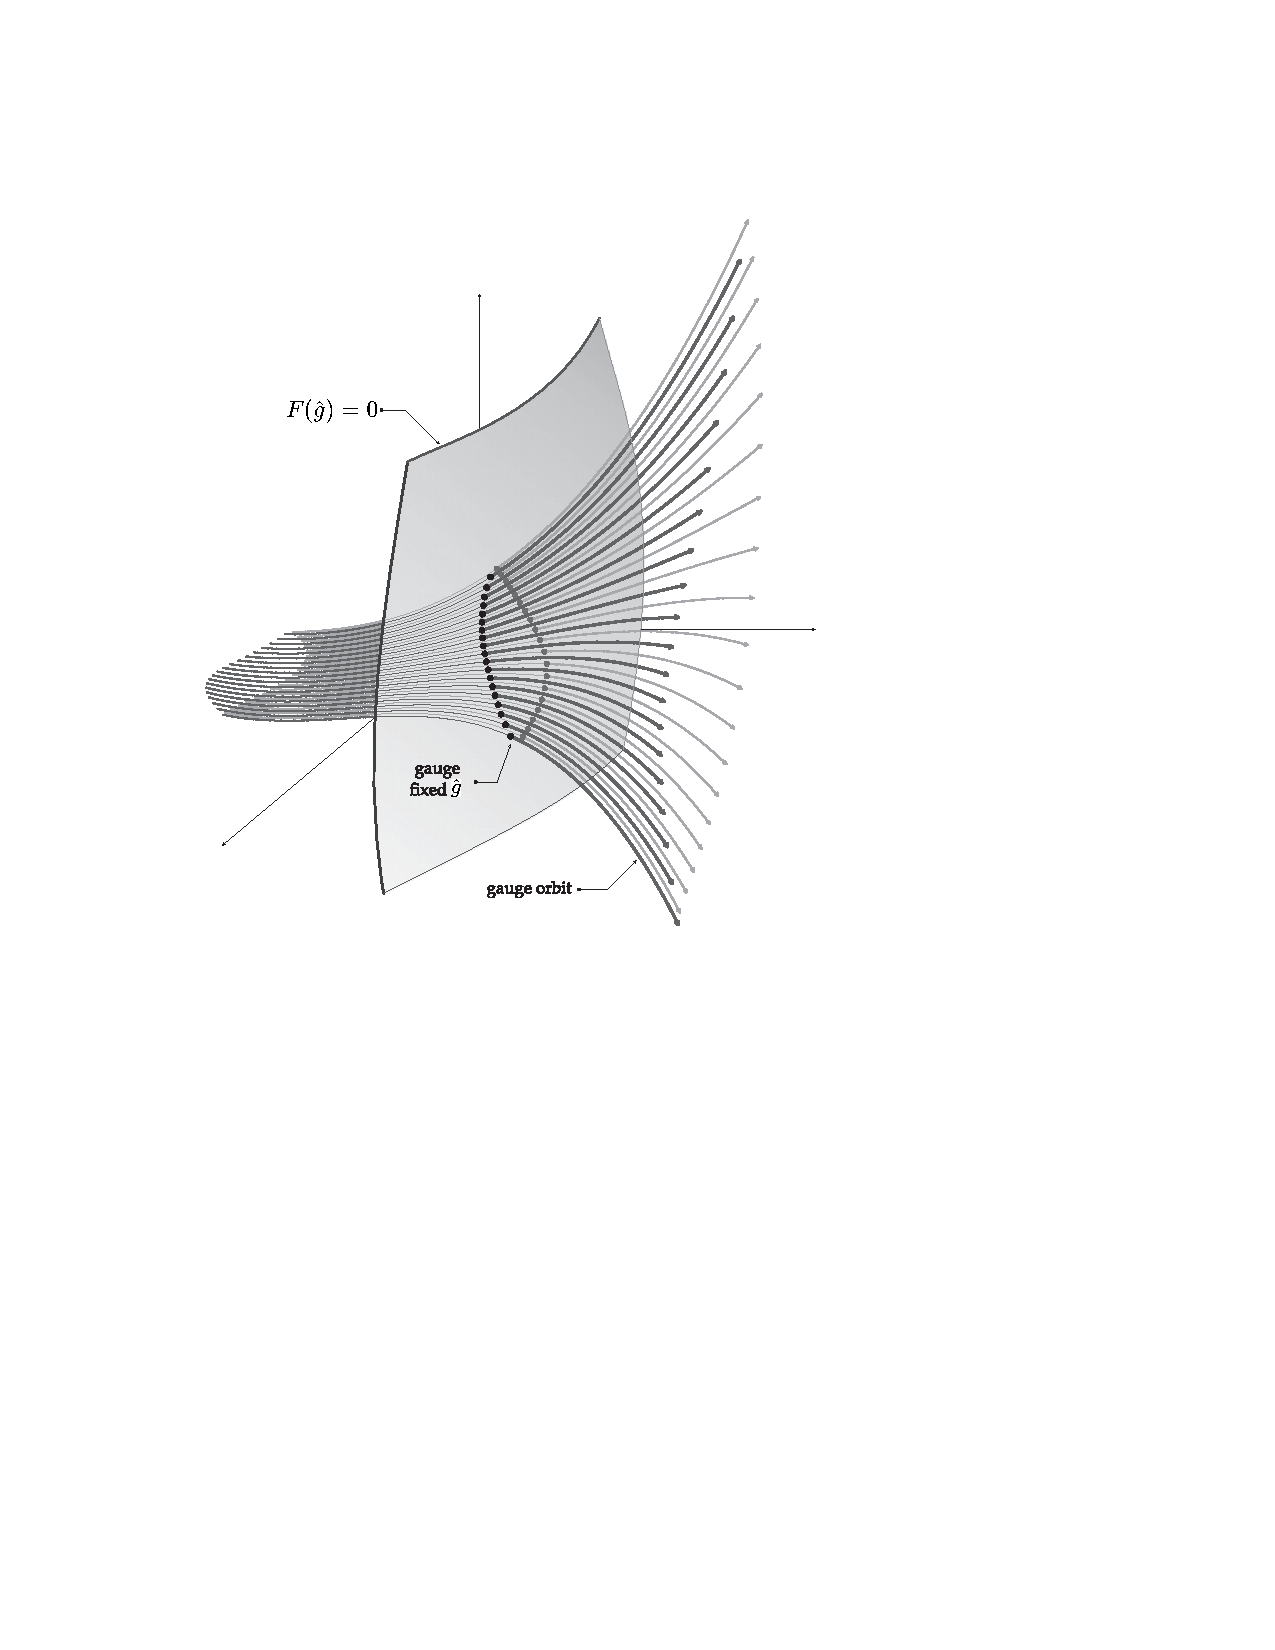
\includegraphics[width=0.5\linewidth]{figs/fig3.pdf}
	\caption{规范固定}
	\label{fig:3}
\end{figure}

虽然前面把$[g]$和复结构对应起来了,这告诉我们路径积分包含模空间的积分,但是为了对$\mathrm{diff}\oplus\mathrm{weyl}$积分,取规范固定$\hat{g}$后完全定下规范了吗?或者说我们建立了和规范变换$\zeta$和$[\hat g]$内元素的一一对应吗?这样$\int [\mathcal{D}\zeta]$才等于$V_{\mathrm{diff}\times\mathrm{weyl}}$从而完全消去规范冗余。但显然不是的,从前面光锥规范就能看出,单纯取等温坐标固定$g$没有完全定下规范,还又共形变换作为$\mathrm{diff}\oplus\mathrm{weyl}$的子群没有固定。同样的,规范变换$\zeta$跑遍了$[\hat g]$中的元素,但是$\mathrm{diff}\oplus\mathrm{weyl}$变换的子群CKG变换$\hat g$后仍得到$\hat g$,也就是说在规范固定点$\hat g$处仍有冗余的规范$V_{\mathrm{CKG}}$没有被消除。在数学上与之相关的群被称为黎曼曲面的自同胚群$\operatorname{Aut}(M)$。如果这个群是离散群,那么只需要除去$n_R=|\operatorname{Aut}(M)|$就可以消去规范,但是如果这个群是连续李群,这对应黎曼曲面$\pi_1(M)$是阿贝尔群的情况\footnote{对应的黎曼曲面称为例外黎曼面。},CKG的消去可以通过固定黎曼面上的某几个点来消去,也就是说规范选取变成了$(\hat g,\hat\sigma_{i\in\mathcal{F}})$,可以解释为固定了其中几个顶角算符的插入点\footnote{本文不考虑顶角算符个数不足以固定插入点的情况。},具体是固定哪几个顶角算符以及固定点的坐标$z_{i\in\mathcal{F}}$并不会影响最终的关联函数结果。自然联想到这种顶角算符的固定是通过积分顶角算符到无积分顶角算符之间的转换实现的,后面会看到的确如此。

上面规范固定的过程可以看作是下面的积分测度变换:
\begin{equation}
	\label{eq:4.4}
	\mathcal{D}gd^{2n}\sigma\to|J|\mathcal{D} \zeta d^{\mu}td^{2n-\kappa}\sigma
\end{equation}
其中$|J|$是变换的雅可比行列式。其中$\mu = \dim\mathfrak{M}_{g,n}$,$\kappa$则是CKG生成元个数。注意,在黎曼曲面上固定一个点需要一个“复”的CKG生成元,也就是一对实的CKG生成元来固定,例外是对于开弦顶角算符,由于其插入点在盘面边界圆周$\operatorname{Re}z=0$,所以只需要一个实的CKG生成元就能固定。后面谈到维数均指复维数。下面来计算几个简单黎曼面的自同胚群。

\begin{boxedtext}[黎曼曲面自同胚群]
	黎曼曲面$M$的自同胚群可以利用其基本群在其泛覆叠空间$\hat M$中的正规化子计算:
	\begin{equation*}
		\operatorname{Aut}(M)\cong N(\pi_1(M))/\pi_1(M),\quad N(G):=\{h\in \operatorname{Aut}(\hat{M})|hGh^{-1}=G\}
	\end{equation*}
\end{boxedtext}
所以首先要对三种不同的泛覆叠空间的自同胚群进行计算,结果如下:
\begin{equation}
	\operatorname{Aut}(\mathbb{CP}^1)\cong PSL(2,\mathbb{C}),\quad
	\operatorname{Aut}(\mathbb{C})\cong \operatorname{Aff}(1,\mathbb{C}),\quad
	\operatorname{Aut}(\mathbb{H})\cong PSL(2,\mathbb{R})
\end{equation}
注意到比如$\mathbb{CP}^1$和$\mathbb{H}$的自同胚群都包含两个连通分支,其中单位元存在的连通分支$\operatorname{Aut}_0(M)$才生成CKG。闭弦树级振幅涉及到球面,对应$\operatorname{Aut}_0(S^2)=SL(2,\mathbb{C})$,其有三个复自由度,所以可以固定球面上三个点。一圈振幅对应环面$\operatorname{Aut}_0(T^2)=\mathcal{T}_\mathbb{C}$,即由复平面上的平移群生成,所以可以在环面上固定一个点。同时离散对称性$\sigma^a\to -\sigma^a$同样不会改变环面上的$\hat{g}$,这个$\mathbb{Z}_2$对称性给出$n_R=2$。开弦树级振幅对应盘面也即上半复平面,对应CKG为$\operatorname{Aut}_0(D_2)\cong SL(2,\mathbb{R})$,有三个实自由度,所以同样可以固定盘面边界上三个顶角算符插入点。

模去共形Killing群后,我们考虑的黎曼曲面$\mathcal{M}_g$变成了带标记点的黎曼曲面$\mathcal{M}_{g,n}$,现在来关注其模空间$\mathfrak{M}_{g,n}$。注意到$\delta_m g_{ab}$与$\mathrm{diff\times weyl}$正交:
\begin{equation}
	\begin{aligned}
		0&=\int d^2\sigma g^{1/2}\delta_mg_{ab}\left[-2(P_1\delta\sigma)^{ab}+(2\delta\omega-\nabla\cdot\delta\sigma)g^{ab}\right]\\
		&=\int d^2\sigma g^{1/2}\left[-2(P_1^T\delta^{\prime}g)_a\delta\sigma^a+\delta_mg_{ab}g^{ab}(2\delta\omega-\nabla\cdot\delta\sigma)\right]\\
		&\Rightarrow  g^{ab}\delta_m g_{ab} =0,\quad (P^T_1\delta_m g)_a=0
	\end{aligned}
\end{equation}
第一个无迹条件自动满足,迹包含在Weyl变换项中,第二个条件说明模空间对应$\ker P^T_1$。另外CKG生成元满足的共形Killing方程可以写为:
\begin{equation}
	(P_1\delta\sigma)_{ab}=0
\end{equation}
所以CKG对应$\ker P_1$,模空间维数与CKG维数之间有如下公式:
\begin{boxedtext}[Riemann-Roch公式]
	\begin{equation}
		\label{eq:4.8}
		\dim\ker P_n-\dim\ker P_n^T=(n+\frac12)\chi=(2n+1)(1-g)
	\end{equation}
\end{boxedtext}
上式\ref{eq:4.8}只是Riemann-Roch定理的一个特例。注意到$\kappa$正好对应黎曼曲面上固定点的个数,所以上述结果可以推广到固定点任意多的黎曼曲面模空间:
\begin{boxedtext}[模空间维数]
	亏格为$g$且带$n$个标记点的黎曼曲面模空间是一个连通光滑的复轨形,维数为:
	\begin{equation}
		\label{eq:4.9}
		\dim\mathfrak{M}_{g,n} = 3 g - 3 + n
	\end{equation}
	且我们考虑$2g-2+n>0$情况,这对应$\operatorname{Aut}(M_{g,n})$是有限群,也即固定点后完全模去了CKG。
\end{boxedtext}
模空间是一个复轨形来源于其有如下的计算方式\footnote{考虑不带标记点的简单情况。}:
\begin{boxedtext}[Teichm\"uller空间]
	$\mathrm{Diff}^+$表示保定向的微分同胚变换,$\mathrm{Diff}_0$表示与单位映射同伦的微分同胚。则定义模群$\Gamma_g$\footnote{也常称为Mapping Class Group。}和Teichm\"uller空间$\mathfrak{T}_g$:
	\begin{equation*}
		\Gamma_\mathrm{g}:=\mathrm{Diff}^+(M)/\mathrm{Diff}_0(M),\quad \mathfrak{T}_\mathrm{g}\equiv\frac{\mathcal{M}_g}{\mathrm{Weyl}(M)\times\mathrm{Diff}_0(M)}
	\end{equation*}
	黎曼曲面模空间有如下轨形形式:
	\begin{equation}
		\label{eq:4.10}
		\mathfrak{M}_\mathrm{g}=\mathfrak{T}_\mathrm{g}/\Gamma_\mathrm{g}
	\end{equation}
\end{boxedtext}
利用\ref{eq:4.9}计算发现球面$g=0,n=3$情况模空间平凡,所以树图振幅不涉及模空间积分的计算。第一个非平凡的例子是环面$g=1,n=1$,模空间维数为$1$,环面上的复结构由下面的格生成:
\begin{equation}
	\Gamma:=\mathbb{Z}\alpha_1+\mathbb{Z}\alpha_2=\{n\alpha_1+m\alpha_2:n,m\in\mathbb{Z}\}
\end{equation}
$T^2 \cong  \mathbb{C}/\Gamma$,$\alpha_{1,2}\in\mathbb{C}$。不同复结构由$SL(2,\mathbb{Z})$意义下不同构的格生成。两个复自由度$\alpha_1,\alpha_2$约化为一个。在\ref{eq:4.10}的观点下,环面的模空间为:
\begin{equation}
	\mathfrak{M}_{1,1}=\mathbb{H}/PSL(2,\mathbb{Z})
\end{equation}
所以模空间参数$\tau$可以通过模群限制在图\ref{fig:5}所示的阴影部分中,即模空间积分范围为:
\begin{equation}
	\mathscr{F}:=\left\{\tau\in\mathscr{H}:-\frac{1}{2}\leq\mathrm{Re}(\tau)\leq\frac{1}{2},|\tau|\geq1\right\}
\end{equation}
这种模空间边界的自然存在性,或者说因为模不变性,让弦论自然拥有一个截断,从而是紫外有限的理论。\cite{Witten:2015mec}
\begin{figure}[htbp]
	\centering
	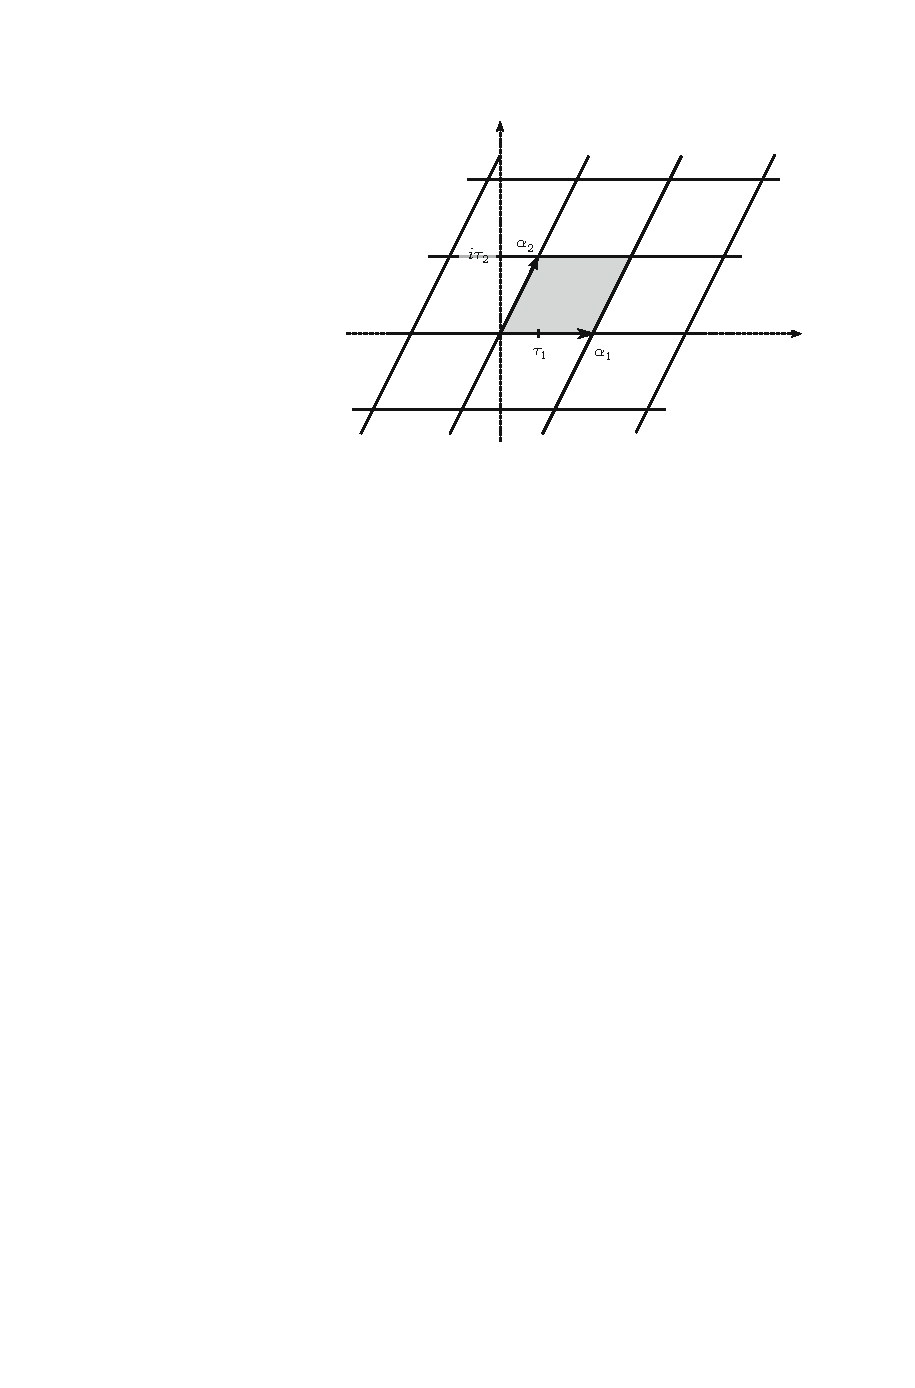
\includegraphics{figs/fig4.pdf}
	\caption{环面上不同的复结构,在$SL(2,\mathbb{Z})$同构的意义下,取$(\alpha_1,\alpha_2)=(1,\tau)$}
	\label{fig:4}
\end{figure}
\begin{figure}[htbp]
	\centering
	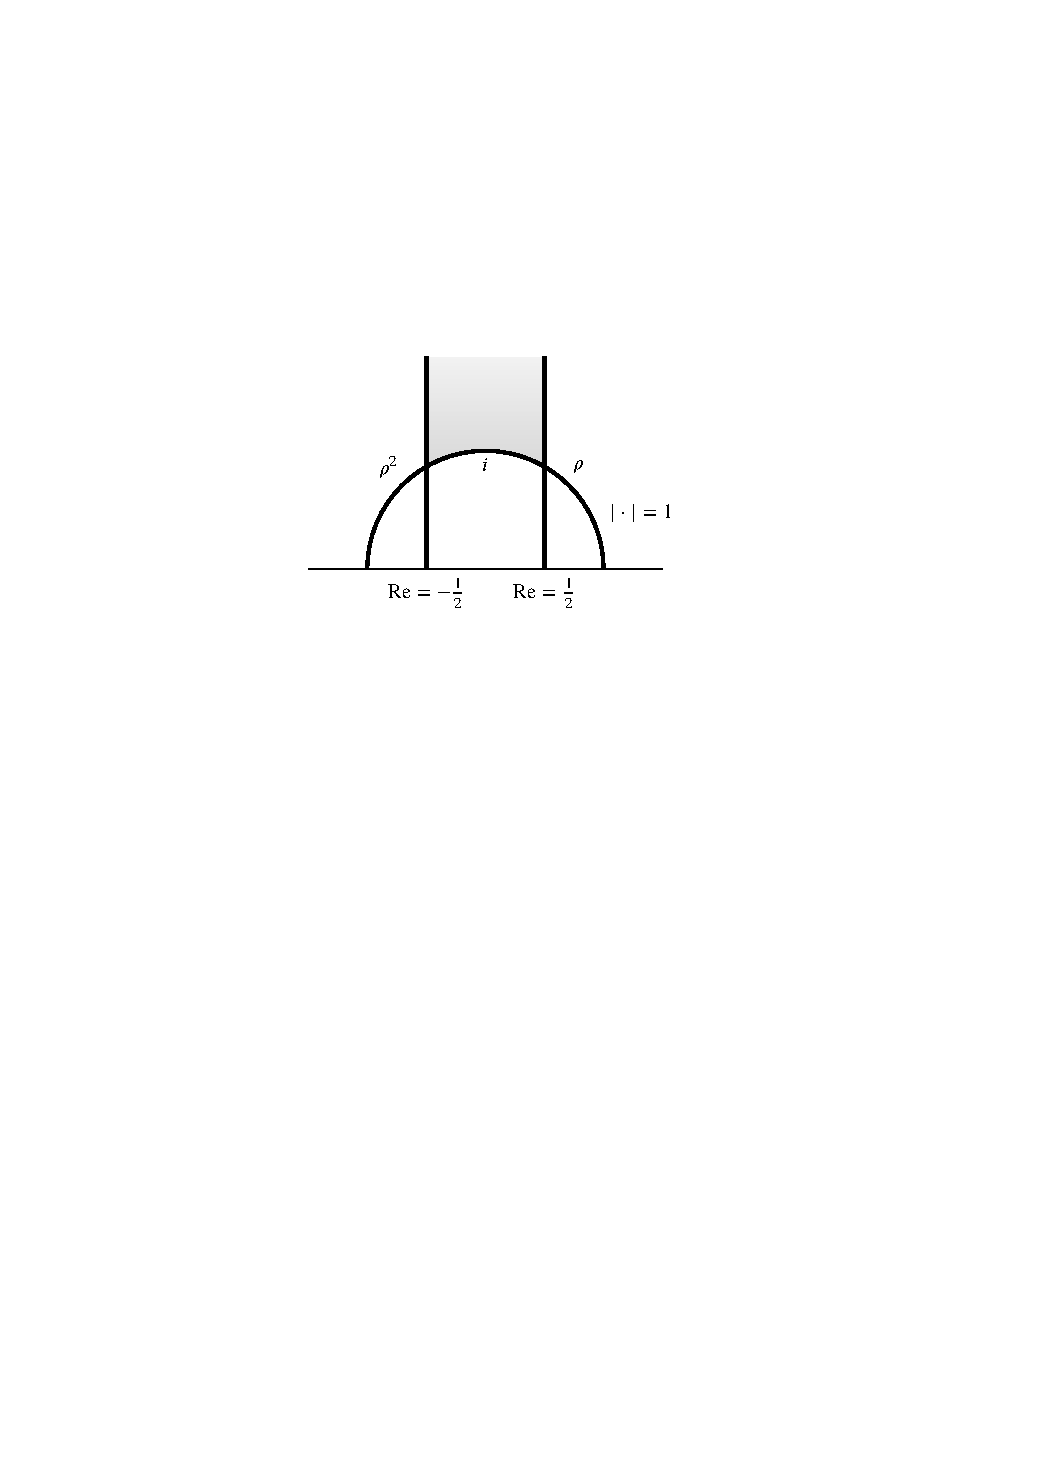
\includegraphics{figs/fig5.pdf}
	\caption{环面模空间的基本域,$\rho:=e^{2\pi i/6}$}
	\label{fig:5}
\end{figure}

在黎曼面上积分的想法近年来也从弦论渗透到了场论振幅计算中,Cachazo-He-Yuan形式给了场论振幅利用带标记点黎曼面上积分的统一形式\cite{Cachazo:2013iea,Cachazo:2013hca}:
\begin{equation}
	\mathcal{A}_{n}^\text{tree}=\int d\mu_{n}\mathcal{I}_{n}^L\mathcal{I}_{n}^R,\quad d\mu_{n}=\frac{d^{n}\sigma}{\mathrm{volSL}(2,\mathbb{C})}{\prod_{a}}^{\prime}\delta{\left(\sum_{b\neq a}\frac{s_{ab}}{\sigma_{ab}}\right)}
\end{equation}
不同场论的区别在于CHY被积函数$\mathcal{I}$,但是树级振幅都有上述的统一形式!
\subsection{FP量子化}
现在来计算\ref{eq:4.4}中的Jacobi行列式,这个积分测度变换对应插入:
\begin{equation}
	1=\Delta_{\mathrm{FP}}(g,\sigma)\int_\mathfrak{M}d^\mu t\int_\mathrm{diff\times Weyl}\mathcal{D}\zeta\delta(g-\hat{g}(t)^\zeta)\prod_{(a,i)\in \mathcal{F}}\delta(\sigma_i^a-\hat{\sigma}_i^{\zeta a})
\end{equation}
利用\ref{eq:4.1}以及标准的FP鬼场方法计算得到:
\begin{equation}
	\label{eq:4.16}
	\Delta_{\text{FP}}=\frac{1}{n_R}\int\mathcal{D}b_{ab}\mathcal{D}c^a\exp(-S_g)\prod_{k=1}^\mu\frac{1}{4\pi}(b,\partial_{t^k}\hat{g})\prod_{(a,i)\in \mathcal{F}}c^a(\hat{\sigma}_i),\quad S_g=\frac{1}{2\pi}\left(b,(\hat{P}_1c)\right)
\end{equation}
当$\hat g$取共形规范时$b_{ab}$和$c^a$退化为全纯和反全纯左右模,也即\ref{eq:2.32}形式。这里涉及到对称无迹张量之间的内积,定义为:
\begin{equation}
	\label{eq:4.17}
	(t,t^\prime)_{\hat g}:=\int d\sigma^a {\hat g}^{\frac{1}{2}} (t\cdot t^\prime)
\end{equation}
这里$\cdot$表示对所有指标缩并。\ref{eq:2.39}规范固定后的形式为:
\begin{equation}
	\label{eq:4.18}
	\begin{aligned}
		S_{j_1...j_n}(k_1,\ldots,&k_n)=\sum_{\substack{\text{worldsheet}\\\text{topologies}}}\int_{\mathfrak{M}}\frac{d^\mu t}{n_R}\mathcal{D}X\mathcal{D}b\mathcal{D}c\exp(-S_\mathrm{m}-S_\mathrm{g}-\lambda\chi)\\&\times\prod_{(a,i)\notin \mathcal{F}}\int d\sigma_i^a\prod_{k=1}^\mu\frac{1}{4\pi}(b,\partial_{t^k}\hat{g})\prod_{(a,i)\in\mathcal{F}}c^a(\hat{\sigma}_i)\prod_{i=1}^n\hat{g}(\sigma_i)^{1/2}U_{j_i}(k_i,\sigma_i)
	\end{aligned}
\end{equation}
由此可见固定顶角算符插入点确实相当于将无积分顶角算符换为积分顶角算符。现在对$bc$进行模展开,将上式与$bc$鬼场零模的插入联系起来。
\begin{equation}
	\label{eq:4.19}
	\begin{gathered}
		c^a(\sigma)=\sum_Jc_J\mathsf{C}_J^a(\sigma),\quad b_{ab}(\sigma)=\sum_Kb_K\mathsf{B}_{Kab}(\sigma)\\
		P_1^TP_1\mathsf{C}_J^a=\mu_J^{2}\mathsf{C}_J^a,\quad P_1P_1^T\mathsf{B}_{Kab}=\nu_K^2\mathsf{B}_{Kab}
	\end{gathered}
\end{equation}
$\mathsf{C}_J$,$\mathsf{B}_{K}$在\ref{eq:4.17}内积的意义下正交归一。而且两者的非零模之间有一一对应:
\begin{equation}
	\mathsf{B}_{Jab}=\frac{1}{\nu_J}(P_1\mathsf{C}_J)_{ab},\quad\nu_J=\mu_J\neq0
\end{equation}
而且零模正好是$\ker P_1^T$和$\ker{P_1}$中的向量。FP行列式\ref{eq:4.16}路径积分可以直接用模展开得到:
\begin{equation}
	\label{eq:4.21}
	\begin{aligned}
		\Delta_{\text{FP}}=&\int\prod_{k=1}^\mu db_{0k}\prod_{j=1}^\kappa dc_{0j}\prod_Jdb_Jdc_J\exp\left(-\frac{\nu_Jb_Jc_J}{2\pi}\right)\prod_{m=1}^\mu\frac{1}{4\pi}(b,\partial_{t^{m}}\hat{g})\prod_{(a,i)\in\mathcal{F}}c^a(\sigma_i)\\
		=&\int\prod_{k=1}^\mu db_{0k}\prod_{m=1}^\mu\left[\sum_{k^{\prime}=1}^\mu\frac{b_{0k^{\prime}}}{4\pi}\left(\mathrm{B}_{0k^{\prime\prime}},\partial_{t^m}\hat{g}\right)\right]
		\int\prod_{j=1}^\kappa dc_{0j}\prod_{(a,i)\in\mathcal{F}}\left[\sum_{j^{\prime}=1}^\kappa c_{0j^{\prime}}\mathsf{C}_{0j^{\prime}}^a(\sigma_i)\right]
		\\
		&\times\int\prod_Jdb_Jdc_J\exp\left(-\frac{\nu_Jb_Jc_J}{2\pi}\right)\\
		=&\det\frac{(\mathsf{B}_{0k},\partial_{t^m}\hat{g})}{4\pi}{\det}\mathsf{C}_{0j}^a(\sigma_i){\det}^{\prime}\left(\frac{P_1^TP_1}{4\pi^2}\right)^{1/2}
	\end{aligned}
\end{equation}
第二个等号利用了格拉斯曼变量积分的性质,只有在被积函数为积分变量的最高形式时才不为零。最后一个等号中${\det}^\prime$表示不考虑零模贡献,否则显然$\det=0$。由上式不难看出规范固定的过程正是插入$bc$鬼场零模,而Riemann-Sroch定理$\mu-\kappa$给出的正是鬼数补偿,其正好补偿背景鬼数\ref{eq:2.66}。

虽然鬼场方法是极具物理思想的方法,但是其推导出来的结果右有非常清晰的物理解释。\ref{eq:4.21}中第三项可以看作是一个归一化系数不用过多考虑,第二项$c$鬼场零模正好对应CKG生成元,第一项在数学上相当于插入一些Beltrami微分,是复结构的体现。而且,单纯从形式上来说\ref{eq:4.18}有下面更简单的形式:\footnote{Beltrami微分定义为$\mu_{ka}^b:=\frac{1}{2}\hat{g}^{bc}\partial_k\hat{g}_{ac}$}
\begin{equation}
	\label{eq:4.22}
	S(1;\ldots;n)=\sum_{\substack{\text{worldsheet}\\\text{topologies}}}e^{-\lambda\chi}\int_F\frac{d^mt}{n_R}\left\langle\prod_{k=1}^m\frac{1}{2\pi}(b,\mu_k)\prod_{i=1}^nc\tilde{c}V\right\rangle
\end{equation}
注意我们将所有的顶角算符插入点全部固定,而增加了Beltrami微分,这也是鬼数补偿的要求。相当于考虑亏格相同,但是固定点更多的模空间:
\begin{equation}
	\mathfrak{M}_{g,n+n_c+n_o},\quad \dim\mathfrak{M} = -\frac32 \chi + \frac12 n_o+n_c
\end{equation}
固定点的信息被转移到了模空间中去。但是从计算的角度上看依旧是\ref{eq:4.18}更方便,因为模空间积分计算比较复杂。

前面都是对玻色弦考虑的,超弦的情况要复杂得多。对于本篇论文,只要知道树图是平凡的,我们只需要关注物质场关联函数计算以及$c$鬼场的插入即可。RNS超弦唯一多要求绘景数求和为$2$。
\section{树级关联函数计算}
本节计算树级物质场和鬼场的关联函数,直接从路径积分出发计算,并说明此结果于OPE计算得到的结果相同。这里我们只对玻色部分物质场进行计算,本章最后计算超弦振幅时会直接使用OPE计算费米部分关联函数。

观察玻色弦顶角算符,需要计算如下物质场关联函数:
\begin{equation}
	\label{eq:4.23}
	\left\langle\prod_{i=1}^n:e^{ik_i\cdot X(z_i,\bar{z}_i)}:\prod_{j=1}^p\partial X^{\mu_j}(z_j^{\prime})\prod_{k=1}^q\bar{\partial}X^{\nu_k}(\bar{z}_k^{\prime\prime})\right\rangle
\end{equation}
注意到:
\begin{equation}
	\label{eq:4.24}
	i\rho_j\cdot\partial Xe^{ik_j\cdot X(z_j)}=\left.\exp\bigg(i[k_j\cdot X(z_j)+\rho_j\cdot\partial X(z_j)]\bigg)\right|_{\text{linear in }\rho_j}
\end{equation}
所以我们只需要计算下面的关联函数即可得到\ref{eq:4.23}:
\begin{equation}
	\label{eq:4.25}
	\left\langle\prod_i:\exp\bigg(i\left[k_{i\mu}X^\mu(z_i)+\rho_{i\mu}\partial X^\mu(z_i)\right]\bigg):\right\rangle
\end{equation}
不妨考虑下面更一般的配分函数计算,$J=0$时即为真空配分函数:
\begin{equation}
	\label{eq:4.26}
	Z\left[J\right]=\left\langle\exp\left(i\int d^2\sigma J(\sigma)\cdot X(\sigma)\right)\right\rangle
\end{equation}
利用类似\ref{eq:4.19}的模展开技巧计算$\mathcal{D}X$:
\begin{equation}
	\begin{gathered}
		X^\mu(\sigma)=\sum_Ix_I^\mu\mathsf{X}_I(\sigma),\quad\nabla^2\mathsf{X}_I=-\omega_I^2\mathsf{X}_I,\quad \mathsf{X}_0=\left(\int d^2\sigma g^{1/2}\right)^{-1/2}\\ \left(\mathsf{X}_I,\mathsf{X}_J\right)=\delta_{IJ},\quad
	\mathsf{J}_I^\mu:=\int d^2\sigma J^\mu(\sigma)\mathsf{X}_I(\sigma)
	\end{gathered}
\end{equation}
带入到\ref{eq:4.26}得到:
\begin{equation}
	\label{eq:4.28}
\begin{aligned}
		Z\left[J\right]=&\prod_{I,\mu}\int dx_I^\mu\exp\left(-\frac{\omega_I^2x_I^\mu x_{I\mu}}{4\pi\alpha^{\prime}}+ix_I^\mu J_{I\mu}\right)\\
	=&i(2\pi)^d\delta^d(\mathsf{J}_0)\prod_{I\neq0}\left(\frac{4\pi^2\alpha^{\prime}}{\omega_I^2}\right)^{d/2}\exp\left(-\frac{\pi\alpha^{\prime}\mathsf{J}_I\cdot \mathsf{J}_I}{\omega_I^2}\right)\\
	=&i(2\pi)^d\delta^d(\mathsf{J}_0)\left({\det}^{\prime}\frac{-\nabla^2}{4\pi^2\alpha^{\prime}}\right)^{-d/2}\exp\left(-\frac{1}{2}\int d^2\sigma d^2\sigma^{\prime}J(\sigma)\cdot J(\sigma^{\prime})G^{\prime}(\sigma,\sigma^{\prime})\right)
\end{aligned}
\end{equation}
其中$G'$表示略去零模贡献的$X^\mu$格林函数:\footnote{对$\mathsf{X}_0$比较形象的解释源于世界面紧致,来源于传播带来的背景荷。}
\begin{equation}
	\label{eq:4.29}
	\begin{gathered}
		G^{\prime}(\sigma_1,\sigma_2)=\sum_{I\neq0}\frac{2\pi\alpha^{\prime}}{\omega_I^2}\mathsf{X}_I(\sigma_1)\mathsf{X}_I(\sigma_2)\\
	-\frac{1}{2\pi\alpha^{\prime}}\nabla^2G^{\prime}(\sigma_1,\sigma_2)=\sum_{I\neq0}\mathsf{X}_I(\sigma_1)\mathsf{X}_I(\sigma_2)=g^{-1/2}\delta^2(\sigma_1-\sigma_2)-\mathsf{X}_0^2
	\end{gathered}
\end{equation}
\ref{eq:4.28}计算中,$x^0_I$应当Wick转动到欧氏空间给出收敛的高斯积分,另外物质场零模需要单独处理,给出$\delta$函数,后面会进一步解释。注意,上面的计算结果原则上可以应用到任意世界面拓扑,只是格林函数有所不同。上式中取:
\begin{equation}
	\label{eq:4.30}
	J(\sigma)=\sum_{i=1}^n\left(k_i-\rho^a_i\partial_a\right)\delta^2(\sigma-\sigma_i)
\end{equation}
便得到了\ref{eq:4.25},但是去掉NOP。加上NOP的过程其实就是重整化的过程,注意到$G'(\sigma,\sigma)\to\infty$,记其不发散的全纯部分为$G^\prime_r$。\ref{eq:4.28}积分中$\sigma=\sigma'$时存在发散,将其重整化为$G^\prime_r(\sigma,\sigma)$发散便消除了。从共形场论的观点来看$G'(\sigma_i,\sigma_j)$是在计算$V_i,V_j$之间的缩并,而$G'(\sigma_i,\sigma_i)$是在计算$V_i$内部的缩并,显然发散,但顶角算符本身是定义在NOP意义下。所以把$G'$替换为$G'_r$就是将OPE重整化为NOP,去掉奇异项就是在去掉NOP内部的缩并。\footnote{回忆在计算NOP的缩并时,等价于不考虑NOP内部缩并,从而去除发散。}下面以球面上的计算为例说明这样做的后果。

取共形规范,在球面上求解\ref{eq:4.29}得到:
\begin{equation}
\begin{gathered}
	\label{eq:4.31}
		G^{\prime}_{S^2}(\sigma_1,\sigma_2)=-\frac{\alpha^{\prime}}{2}\ln|z_{12}|^2+f(z_1,\bar{z}_1)+f(z_2,\bar{z}_2)\\
	f(z,\bar{z})=\frac{\alpha^{\prime}\mathsf{X}_0^2}{4}\int d^2z^{\prime}\ln|z-z^{\prime}|^2+\mathrm{const}
\end{gathered}
\end{equation}
显然$G'$被分为奇异部分和全纯部分$G'_r$,为了简单起见取$\ref{eq:4.30}$中$\rho = 0$:
\begin{equation}
	\label{eq:4.32}
\begin{aligned}
		&\left\langle:e^{ik_1\cdot X(\sigma_1)}::e^{ik_2\cdot X(\sigma_2)}:\ldots:e^{ik_n\cdot X(\sigma_n)}:\right\rangle_\mathrm{S_2}\\
	=&iC_{S_2}^X(2\pi)^d\delta^d(\sum_ik_i)\times\exp\left(-\frac12\sum_{\substack{i,j=1\\i\neq j}}^nk_i\cdot k_jG^{\prime}(\sigma_i,\sigma_j)-\frac{1}{2}\sum_{i=1}^nk_i^2G_r^{\prime}(\sigma_i,\sigma_i)\right)
\end{aligned}
\end{equation}
不难发现物质场零模积分给出的$\delta$函数正好就是动量守恒,其中归一化常数将$\delta(\mathsf{J}_0)$的Jacobi行列式吸收后定义为:
\begin{equation}
	C_{S_2}^X=\mathsf{X}_0^{-d}\left({\det}^{\prime}\frac{-\nabla^2}{4\pi^2\alpha^{\prime}}\right)_{S_2}^{-d/2}
\end{equation}
这个归一化系数一般和模空间参数有关,而树图不涉及模空间积分,所以此归一化系数连带动量守恒$i(2\pi)^d\delta^d(\sum_i k_i)$在后续计算中全部略去。再利用$\ref{eq:4.31}$不难发现$f(z,\bar z)$贡献的项都$\propto\sum_i k_i$。从这个例子可以看出,在重整化加上NOP之后,只有格林函数的奇异部分会对关联函数有贡献,且求和时抛去$\sigma=\sigma'$的奇异项。而格林函数的奇异部分又正好对应OPE,也就是说(至少对于树图)关联函数的非零模部分积分可以直接由OPE计算奇异部分给出,而非奇异部分给出动量守恒$\delta$函数。这与球面上亚纯函数只与奇异性有关相吻合。前面计算是左右模共同的结果,球面上左右模独立传播,取全纯部分给出\ref{eq:4.25}结果:
\begin{equation}
	\label{eq:4.34}
	\prod_{i<j}(z_i-z_j)^{\frac{\alpha^{\prime}}{2}k_i\cdot k_j}\exp\left\{\frac{\alpha^{\prime}}{2}\sum_{i<j}\frac{\rho_i\cdot\rho_j}{(z_i-z_j)^2}+\frac{\alpha^{\prime}}{2}\sum_{i\neq j}\frac{k_j\cdot\rho_i}{(z_i-z_j)}\right\}
\end{equation}
乘上厄米共轭便得到左右模共同贡献,即关联函数:
\begin{equation}
	\left\langle\prod_i:\exp\bigg(i\left[k_{i\mu}X^\mu(z_i,\bar z_i)+\rho_{i\mu}\partial X^\mu(z_i)+\bar\rho_{i\mu}\bar\partial X^\mu(\bar z_i)\right]\bigg):\right\rangle
\end{equation}
利用\ref{eq:4.24}的技巧便可以得到振幅计算中物质场关联函数。同样的思路,下面考虑盘面情况。现在需要在有$\operatorname{Im} z = 0$的边界范围内求解\ref{eq:4.29},可以利用电像法求解,$\mathsf{X}_0$零模只贡献给非奇异部分,对最终关联函数无影响,可以扔掉:\footnote{这里使用$\sim$是为了指出格林函数原本应当还包含非奇异部分。}
\begin{equation}
	\label{eq:4.36}
	G^{\prime}_{D^2}(\sigma_1,\sigma_2)\sim-\frac{\alpha^{\prime}}{2}\ln|z_1-z_2|^2-\frac{\alpha^{\prime}}{2}\ln|z_1-\overline{z}_2|^2\overset{\operatorname{Im} z = 0}{\sim} -2\alpha^\prime \ln|y_1-y_2|
\end{equation}
\begin{figure}[htbp]
	\centering
	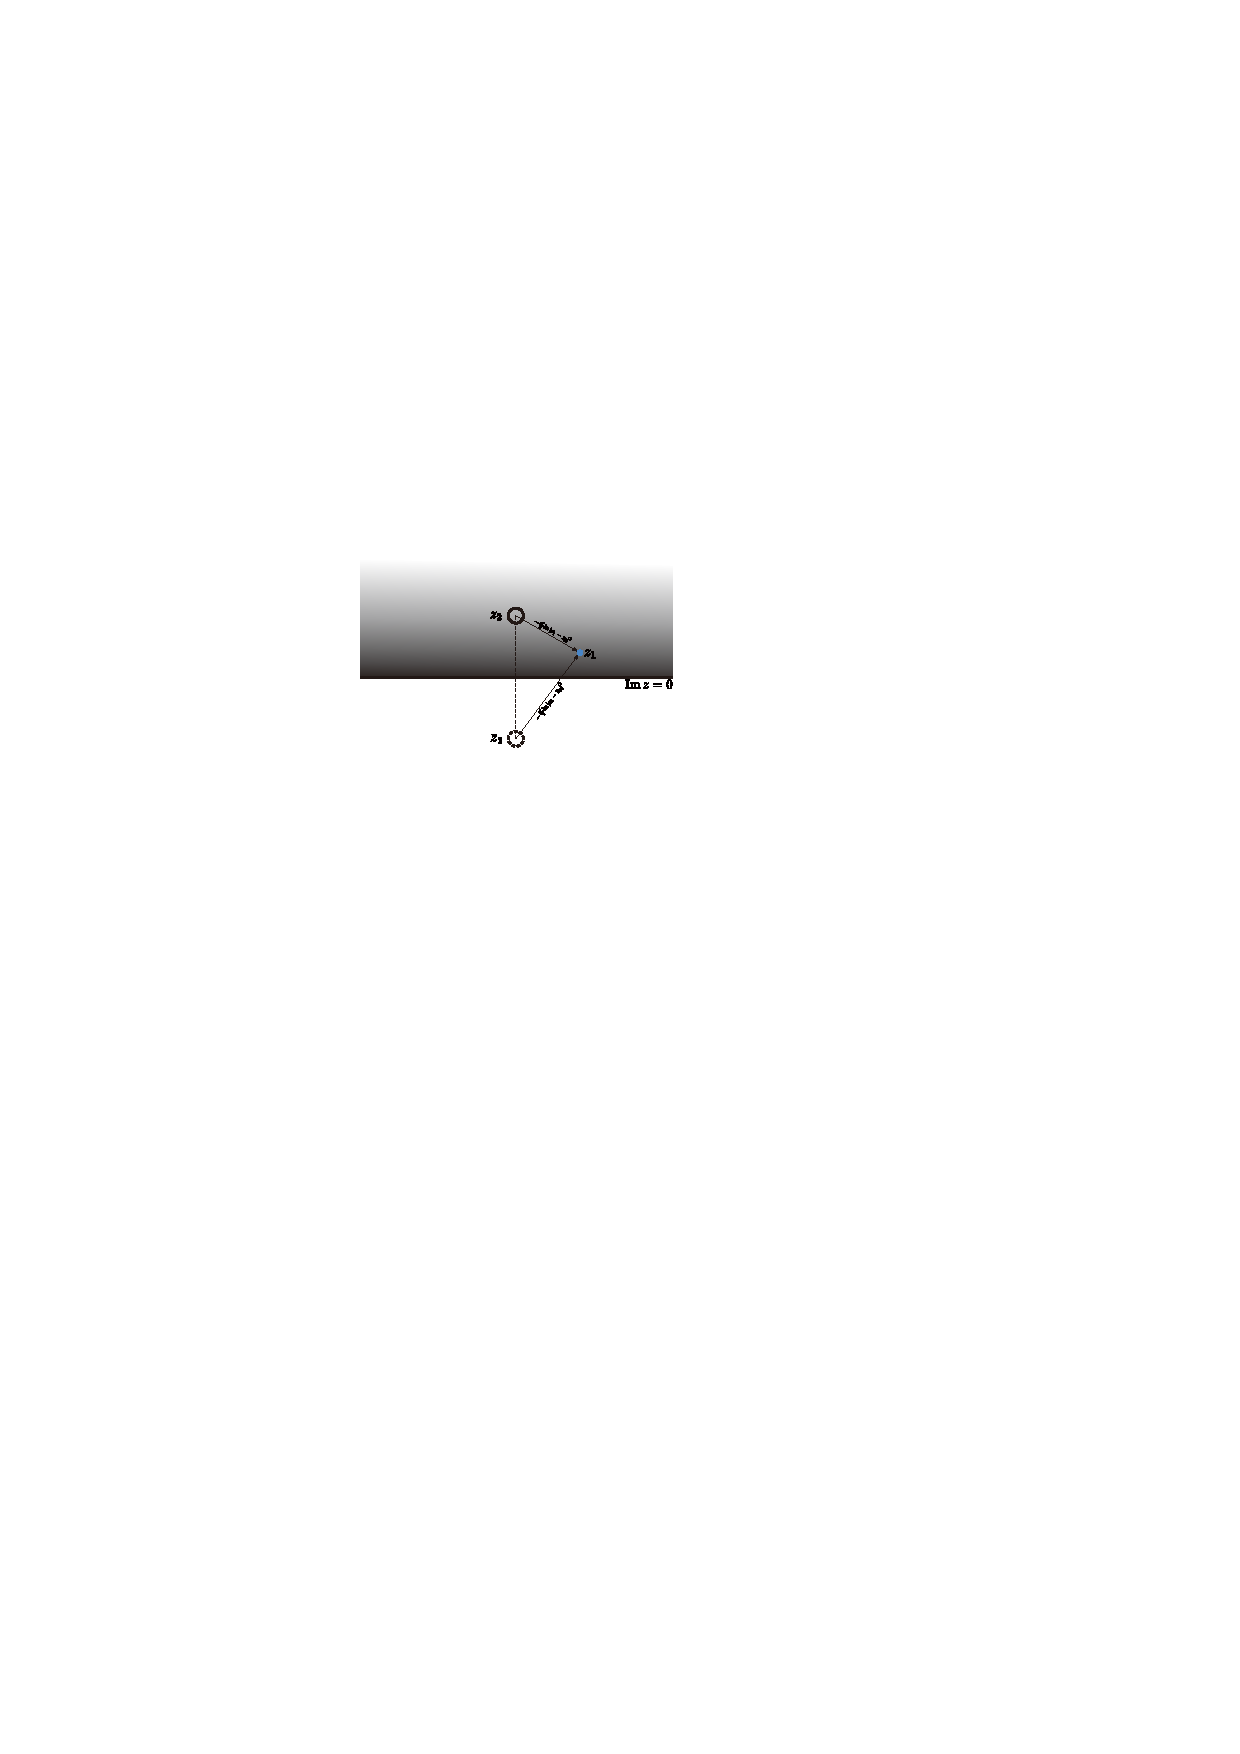
\includegraphics[width=0.8\linewidth]{figs/fig6.pdf}
	\caption{电像法计算格林函数}
	\label{fig:6}
\end{figure}
类似\ref{eq:4.32}的计算并注意到顶角算符均在实轴上插入:
\begin{equation}
	\label{eq:4.37}
	\begin{aligned}
		&\left\langle\prod_{i=1}^n :\exp\bigg(i\left[k_i\cdot X(y_i)+\rho_{i\mu}\partial X^{\mu}(y_i)\right]\bigg):\right\rangle_{D_2}\\
	=&\prod_{i<j}(y_i-y_j)^{2{\alpha^{\prime}}k_i\cdot k_j}\exp\left\{2{\alpha^{\prime}}\sum_{i<j}\frac{\rho_i\cdot\rho_j}{(y_i-y_j)^2}+2\alpha^{\prime}\sum_{i\neq j}\frac{k_j\cdot\rho_i}{(y_i-y_j)}\right\}
	\end{aligned}
\end{equation}
和\ref{eq:4.34}差别仅是$\alpha^\prime\to4\alpha^\prime$,$z\to y$。\ref{eq:4.34}和\ref{eq:4.37}指数项前面的因子是单纯平面波插入的关联函数,称为Koba-Nielsen因子。正如前面强调的,这些关联函数也可以直接从OPE出发计算。

剩下的就是鬼场关联函数,其实\ref{eq:4.21}就是在算剩下的鬼场关联函数,虽然从OPE来看非零模部分(如果没有$b$插入)无贡献,但是零模部分贡献非平凡。球面上\ref{eq:4.21}第一项由于模空间平凡所以无贡献,第三项是个归一化系数,记作$C^g_{S^2}$,所以只有$c$鬼场零模有贡献:
\begin{equation}
\begin{aligned}
		&\left\langle c(z_1)c(z_2)c(z_3)\tilde{c}(\bar{z}_4)\tilde{c}(\bar{z}_5)\tilde{c}(\bar{z}_6)\right\rangle_{S_2}\\
	\sim&\det\begin{vmatrix}1&1&1\\z_1&z_2&z_3\\z_1^2&z_2^2&z_3^2\end{vmatrix}\det\begin{vmatrix}1&1&1\\\bar{z}_4&\bar{z}_5&\bar{z}_6\\\bar{z}_4^2&\bar{z}_5^2&\bar{z}_6^2\end{vmatrix}=z_{12}z_{13}z_{23}\bar{z}_{45}\bar{z}_{46}\bar{z}_{56}
\end{aligned}
\end{equation}
上式可推广到球面上任意多个$b,c$鬼场插入:
\begin{equation}
	\left\langle\prod_{i=1}^{p+3}c(z_i)\prod_{j=1}^pb(z_j^{\prime})\cdot\widetilde{(\bullet)}\right\rangle_{S_2}=C^g_{S^2}\prod_{\substack{i,i^{\prime}=1\\i<i^{\prime}}}^{p+3}z_{ii^{\prime}}\prod_{\substack{j,j^{\prime}=1\\j<j^{\prime}}}^pz_{jj^{\prime}}^{\prime}\prod_{i=1}^{p+3}\prod_{j=1}^p(z_i-z_j^{\prime})^{-1}
\end{equation}
不难看到分母对应OPE给出非零模积分贡献,分子则来源于$c$鬼场零模贡献。对于开弦,左右模非独立传播,取上式的全纯部分即可。至此,我们已得到计算树级玻色弦振幅所需的所有关联函数,而超弦树级振幅关联函数由于涉及到自旋场还要麻烦些。

最后再来看另外一种计算鬼场关联函数的方法,这种视角在后面考虑纯旋量超弦时很有用,这里单纯以左模为例。前面\ref{eq:2.62}对鬼场真空进行了修正,在计算真空关联函数时,都要对真空泡泡图归一化,比如$SL(2,\mathbb{C})$真空$\braket{1}=1$。但是对于鬼场关联函数,必须要对真空背景鬼数进行补偿,所以其实$\braket{1}=0$,而鬼场修正后的真空应当归一化为$\braket{0}=1$。但是\ref{eq:2.62}给出了两个真空,应当归一化哪一个?其实无所谓,因为他们两个是厄米共轭的,也就是说:
\begin{equation}
	(c_1|1\rangle)^\dagger=\ket{c}^\dagger = \bra{(\partial c c)}=\langle1|c_{-1}c_0
\end{equation}
这是前面提到的鬼数流反常带来的效应,只有这样,合起来补偿鬼数$+3$,关联函数才不为零。那么,鬼场真空归一化应当表示:
\begin{equation}
	\label{eq:bc_norm}
	-\left\langle (c\partial c\partial^2c)(0)\right\rangle = \bra{1}c_{-1}c_0c_1\ket{1}=1
\end{equation}
由此便可以计算:
\begin{equation}
\begin{aligned}
		\left\langle c(z_1)c(z_2)c(z_3)\right\rangle &= \left\langle \left(\sum_{n=0}^\infty \frac{\partial^nc(0)}{n!}z_1^n\right) \left(\sum_{n=0}^\infty \frac{\partial^nc(0)}{n!}z_2^n\right)\left(\sum_{n=0}^\infty \frac{\partial^nc(0)}{n!}z_3^n\right)\right\rangle\\
		&=\left(z_1^2 z_2 - z_1 z_2^2 - z_1^2 z_3 + z_2^2 z_3 + z_1 z_3^2 - z_2 z_3^2\right)\cdot \left(-\frac12\left\langle (c\partial c\partial^2c)(0)\right\rangle\right)\\
	&= z_{12}z_{13}z_{23}\cdot\left(-\frac12\left\langle (c\partial c\partial^2c)(0)\right\rangle\right)\sim z_{12}z_{13}z_{23}
\end{aligned}
\end{equation}
差一个归一化常数,只需要更改一下真空归一化即可,这是无关紧要的。
\section{玻色弦振幅}
\label{sec:4.3}
下文中用$\mathcal{A}$表示开弦树级振幅,$A$表示其色序振幅,$\mathcal{M}$表示闭弦树级振幅。类似Yang-Mills理论,Chan-Paton因子给出开弦树级振幅的色分解:
\begin{equation}
	\mathcal{A}_n=\sum_{\rho\in S_{n-1}}\mathrm{Tr}(\lambda^{a_{\rho(1)}}\lambda^{a_{\rho(2)}}\ldots \lambda^{a_{\rho(n-1)}}\lambda^{a_{n}})\times A(\rho(1),\rho(2),\ldots,\rho(n-1),n)
\end{equation}
色排序振幅指对世界面坐标积分时的某个顺序的贡献,比如$A(1,2,\ldots,n)$就代表$z_1<z_2<\cdots<z_n$的积分贡献。后面我们取规范固定$\{z_1,z_{n-1},z_n\}=\{0,1,\infty\}$,但是这不足以在$SL(2,\mathbb{R})$变换后得到所有色序,因为$SL(2,\mathbb{R})$变换保色序。比如上面的规范固定就一定是$z_1<z_{n-1}<z_n$\footnote{注意由于积分在盘面上,而不是真正在实轴上积分,或者说积分是在一维实射影空间中进行,所有的$<$都要在模去轮换的意义下理解。}。但显然还有$z_{n-1}<z_1<z_n$这种顺序,在这种色序下,取规范固定$\{z_1,z_{n-1},z_n\}=\{1,0,\infty\}$。闭弦规范固定就不涉及到这种顺序性,直接取$\{z_1,z_{n-1},z_n\}=\{0,1,\infty\}$即可。
\subsection{Veneziano 振幅}
考虑四快子振幅,其包含六个色序,如图\ref{fig:7}:
\begin{figure}[htbp]
	\centering
	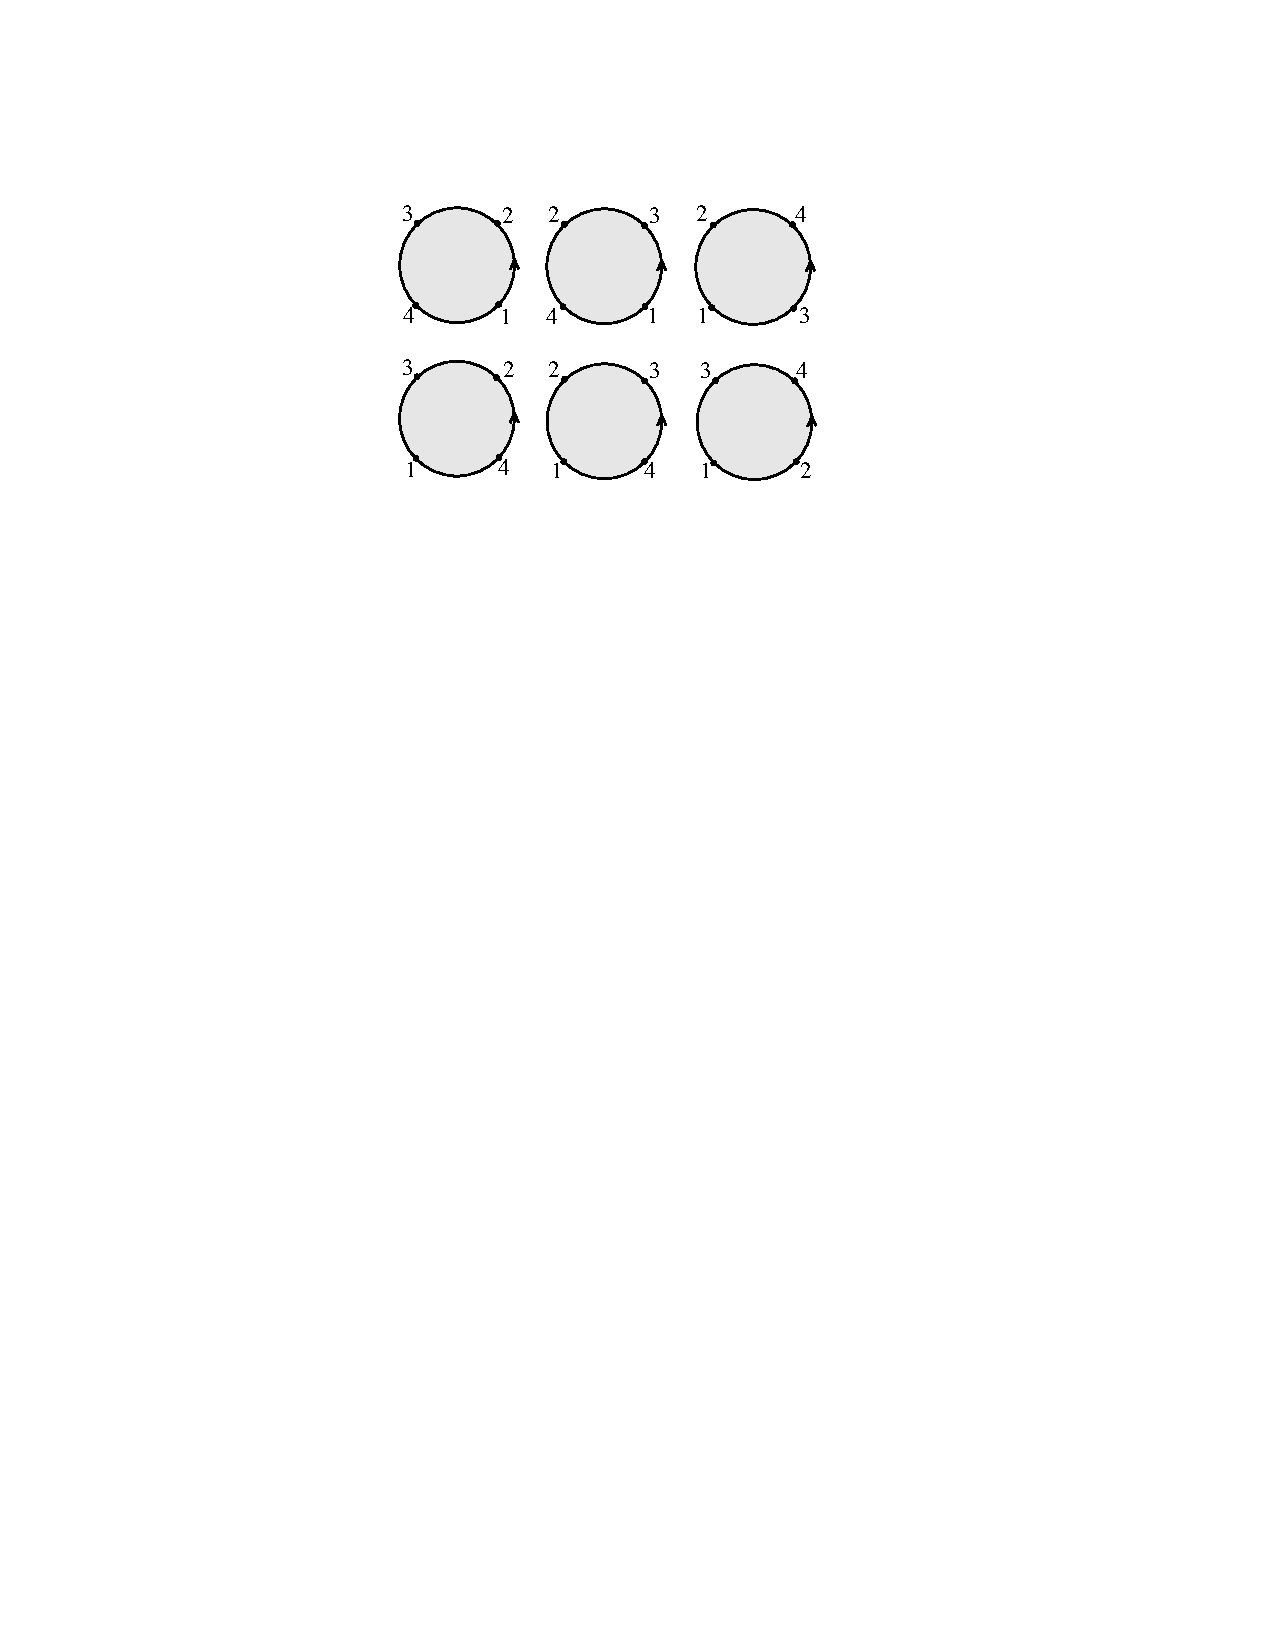
\includegraphics{figs/fig7.pdf}
	\caption{Veneziano振幅的六种色排序,上面三种取$\{z_1,z_{3},z_4\}=\{0,1,\infty\}$,下面三种取$\{z_1,z_3,z_4\}=\{1,0,\infty\}$。箭头方向表示正方向,越过$4$时由$+\infty\to - \infty$}
	\label{fig:7}
\end{figure}
\begin{equation}
\begin{aligned}
		&\mathcal{A}_4(\{T,a\}) \sim \left\langle\prod_{i=1,3,4}: c(y_i)e^{ik_i\cdot X(y_i)}:\int dy_2 e^{ik_2\cdot X(y_2)}\right\rangle\otimes \text{Chan-Paton}\\
	\sim&\int_{0}^1dy_2\mathcal{K}(\{0,1,\infty\};y_2)\operatorname{Tr}\left(\lambda^{a_1a_2a_3a_4}\right)+\int_{1}^\infty dy_2\mathcal{K}(\{0,1,\infty\};y_2)\operatorname{Tr}\left(\lambda^{a_1a_3a_2a_4}\right)\\
	&+\int_{-\infty}^0dy_2\mathcal{K}(\{0,1,\infty\};y_2)\operatorname{Tr}\left(\lambda^{a_2a_1a_3a_4}\right)+\int_{-\infty}^0 dy_2\mathcal{K}(\{1,0,\infty\};y_2)\operatorname{Tr}\left(\lambda^{a_2a_3a_1a_4}\right)\\
	&+\int_{0}^1dy_2\mathcal{K}(\{1,0,\infty\};y_2)\operatorname{Tr}\left(\lambda^{a_2a_3a_1a_4}\right)+\int_{1}^\infty dy_2\mathcal{K}(\{1,0,\infty\};y_2)\operatorname{Tr}\left(\lambda^{a_3a_1a_2a_4}\right)\\
\end{aligned}
\end{equation}
其中$\lambda^{abcd}:=\lambda^a\lambda^b\lambda^c\lambda^d$:
\begin{equation}
	\label{eq:4.42}
	\mathcal{K}(\{a_1,a_2,a_3\};y_2):=\lim_{\{y_1,y_3,y_4\}\to\{a_1,a_2,a_3\}}|y_{13}y_{14}y_{34}|\prod_{i<j}|y_{ij}|^{2\alpha^{\prime}k_i\cdot k_j}
\end{equation}
代入规范固定直接计算得到:
\begin{equation}
	\label{Veneziano}
\begin{aligned}
		\mathcal{A}_4(\{T,a\}) \sim&
	\operatorname{Tr}\left(\lambda^{a_1}\lambda^{a_2}\lambda^{a_4}\lambda^{a_3}+\lambda^{a_1}\lambda^{a_3}\lambda^{a_4}\lambda^{a_2}\right)B(-\alpha_0(s),-\alpha_0(t))\\
	&+\operatorname{Tr}\left(\lambda^{a_1}\lambda^{a_3}\lambda^{a_2}\lambda^{a_4}+\lambda^{a_1}\lambda^{a_4}\lambda^{a_2}\lambda^{a_3}\right)B(-\alpha_0(t),-\alpha_0(u))\\
	&+\operatorname{Tr}\left(\lambda^{a_1}\lambda^{a_2}\lambda^{a_3}\lambda^{a_4}+\lambda^{a_1}\lambda^{a_4}\lambda^{a_3}\lambda^{a_2}\right)B(-\alpha_0(s),-\alpha_0(u))
\end{aligned}
\end{equation}
其中$B$是Beta函数:
\begin{equation}
\begin{gathered}
		B(a,b)=\int_0^1dyy^{a-1}(1-y)^{b-1},\quad \alpha_o(x):= 1+\alpha' x\\
	s=-(k_1+k_2)^2,\quad t=-(k_1+k_3)^2,\quad u=-(k_1+k_4)^2
\end{gathered}
\end{equation}
\ref{Veneziano}就是Veneziano振幅\footnote{原始版本的不带色序,上式中所有迹贡献$1$。}。它是弦理论的第一个公式,原本是强相互作用的经验公式,后面才发现与快子振幅相关\cite{limiao}。早期这个公式有一个与场振幅截然不同的性质,对场振幅而言,四点树级振幅应当是s,t,u三个衰变道的求和。但弦振幅中不涉及到这种求和,换句话说,\ref{Veneziano}可以按照s,t或u的极点展开,极点位置正好是中间传播子在壳即满足\ref{eq:2.16}。但这三个道的展开是一样的,并不像场论中是不一样的展开,求和之后才是完整的振幅。所以弦振幅计算免去了场振幅中对所有费曼图求和的步骤,或者说弦振幅只需要计算一张图就可以了\footnote{当然这张图的计算麻烦得多。},一张图就包含了低能有效场论所有费曼图求和的信息。自然弦振幅也不涉及到场振幅中不同费曼图之间紫外发散的抵消。
\subsection{Virasoro-Shapiro振幅}
Virasoro-Shapiro振幅就是闭弦四快子振幅:
\begin{equation}
	\label{eq:4.45}
	\mathcal{M}_4(\{T\}) \sim \frac{2\pi\Gamma(-\frac{s}{4}-1)\Gamma(-\frac{u}{4}-1)\Gamma(-\frac{t}{4}-1)}{\Gamma(2+\frac{s}{4})\Gamma(2+\frac{u}{4})\Gamma(2+\frac{t}{4})}
\end{equation}
计算中需要用到如下公式:
\begin{equation}
	\int d^2_\mathbb{C}z|z|^{2a-2}|1-z|^{2b-2}=\frac{2\pi\Gamma(a)\Gamma(b)\Gamma(c)}{\Gamma(1-a)\Gamma(1-b)\Gamma(1-c)},\quad a+b+c=1
\end{equation}

现实世界不存在快子态,第一个非平凡的例子是三胶子振幅,其$\operatorname{Tr}(\lambda^{a_1}\lambda^{a_2}\lambda^{a_3})$的色序振幅有如下形式:
\begin{equation}
	\label{eq:4.47}
	A_3^{\text{gluon}}(1,2,3)\sim[(\varepsilon_1\cdot\varepsilon_2)(\varepsilon_3\cdot p_1)+\operatorname{cyc}(1,2,3)]+2\alpha^{\prime}(\varepsilon_1\cdot p_2)(\varepsilon_2\cdot p_3)(\varepsilon_3\cdot p_1)
\end{equation}
显然在$\alpha'\to 0$时就是Yang-Mills理论中(色序)三顶角费曼规则,$\alpha'$的存在暗示弦论的低能有效作用量中存在$\operatorname{Tr}(F^{n>2})$的高阶相互作用量。利用振幅的$\alpha'$展开计算弦论低能有效作用量也是目前弦振幅研究的重要前沿问题。而且由于弦振幅涉及到众多解析数论中的特殊函数,所以这一研究也和数学有很深刻的联系\cite{10.1007/978-3-030-37031-2_4,Stieberger:2016xhs}。

类似的,也可以有开弦闭弦混合振幅,开弦顶角算符在盘面边界圆周上插入,闭弦顶角算符在盘面内部插入,内部插入点积分范围为$|z|<1$。本文主要考虑纯开弦或纯闭弦振幅。文献\cite{dyj,Stieberger:2009hq}考虑了盘面开弦闭弦混合振幅及其与纯开弦振幅的关系。

\section{弦振幅之间的关系}
\subsection{单值关系}
开弦的色序振幅显然有轮换对称性以及:
\begin{equation}
	A_n^{\text{tree}}(1,2,\ldots,n)=(-1)^nA_n^{\text{tree}}(n,\ldots,2,1)
\end{equation}
本节的目的是给出非平凡的色序振幅之间的关系。而且单值关系完全只依赖于Koba-Nielsen因子的解析性质,和具体的顶角算符贡献无关。考虑四点情况,六种色序中有三种拥有相同的Koba-Nielsen因子\ref{eq:4.42},取$\{y_1,y_3,y_4\}={0,1,\infty}$,得到\footnote{也可以选$\{y_1,y_3,y_4\}={1,0,\infty}$规范固定下的另外三种色序得到额外的关系。}:
\begin{equation}
\begin{aligned}
	A_4(1,2,3,4)&=\int_0^1dy_2~|y_2|^{2\alpha^{\prime}k_1\cdot k_2}|1-y_2|^{2\alpha^{\prime}k_2\cdot k_3}\mathcal{V}_4(y_2)\\
	A_4(1,3,2,4)&=\int_1^\infty dy_2~|y_2|^{2\alpha^{\prime}k_1\cdot k_2}|1-y_2|^{2\alpha^{\prime}k_2\cdot k_3}\mathcal{V}_4(y_2)\\
	A_4\left(2,1,3,4\right)&=\int_{-\infty}^{0}dy_2~|y_2|^{2\alpha^{\prime}k_{1}\cdot k_{2}}|1-y_2|^{2\alpha^{\prime}k_{2}\cdot k_{3}}\mathcal{V}_4(y_2)
\end{aligned}
\end{equation}
这里$\mathcal{V}$表示顶角算符插入的贡献\footnote{这里利用了一个技巧,对于快子,前面的因子是正确的,但对于一般的顶角算符,由于固定点的位置完全是任意的,所以应当会贡献$|y_4|^\#$与Koba-Nielsen因子中的$|y_4|$幂次相抵消。否则$|y_4|\to\infty$时奇异。}。由于$\mathcal{V}$极点都在实轴上,而且按照大圆弧引理无穷远处围道贡献为$0$,得到:
\begin{equation}
\begin{aligned}
		0&=\lim_{\epsilon\to0^+}\int_{-\infty+i\epsilon}^{+\infty+i\epsilon}dy_2|y_2|^{2\alpha^{\prime}k_1\cdot k_2}|1-y_2|^{2\alpha^{\prime}k_2\cdot k_3}\mathcal{V}_4(y_2)\\
	&=\left(e^{2\pi i \alpha' k_1\cdot k_2}\int_{-\infty}^0+\int_0^1+e^{-2\pi i \alpha' k_2\cdot k_3}\int_1^\infty\right)\mathrm{d}y_2|y_2|^{2\alpha^{\prime}k_1\cdot k_2}|1-y_2|^{2\alpha^{\prime}k_2\cdot k_3}\mathcal{V}_4(y_2)\\
	&= e^{2\pi i \alpha' k_1\cdot k_2}A_4(2,1,3,4)+A_4(1,2,3,4)+e^{-2\pi i \alpha' k_2\cdot k_3}A_4(1,3,5,4)
\end{aligned}
\end{equation}
这里利用了绝对值在复平面上是多值函数,$\mathrm{e}^{-i\pi}$是因为$|1-y_2|$中$y_2$前的负号,所以相对$y_2$而言$(1,+\infty)$的积分是从实轴下面绕的。更一般的单值关系为:
\begin{equation}
	\label{eq:4.51}
\begin{gathered}
		A_n(\beta,1,\alpha,n)=(-1)^{|\beta|}\operatorname{Re}\left[\prod_{1\leq i<j\leq |\beta|}e^{2i\pi\alpha^{\prime}(k_{\beta_i}\cdot k_{\beta_j})}\sum_{\sigma\in\alpha\shuffle \beta^T}\prod_{i=0}^{|\alpha|}\prod_{j=1}^{|\beta|}e_\sigma^{(\alpha_i,\beta_j)}A_n(1,\sigma,n)\right]\\
	0=\operatorname{Im}\left[\prod_{1\leq i<j\leq |\beta|}e^{2i\pi\alpha^{\prime}(k_{\beta_i}\cdot k_{\beta_j})}\sum_{\sigma\in\alpha\shuffle \beta^T}\prod_{i=0}^{|\alpha|}\prod_{j=1}^{|\beta|}e_\sigma^{(\alpha_i,\beta_j)}\mathcal{A}_n(1,\sigma,n)\right]
\end{gathered}
\end{equation}
其中,定义:
\begin{equation}
	e^{(\alpha,\beta)}_{\sigma}:=\begin{cases} e^{2i\pi\alpha^{\prime}(k_\alpha\cdot k_\beta)},\alpha\succ_\sigma\beta\\1\end{cases}
\end{equation}
$\succ_{\sigma}$表示在排序$\sigma$中的先后顺序。$a\shuffle b$表示洗牌序,也就是$a$和$b$并起来排序,但是排序时保持$a$,$b$各自内部元素的相对顺序。由于$A_n$是盘面上实轴积分,所以总可以选取振幅前的相位因子使其为实数,利用这一点我们将\ref{eq:4.51}拆分为了实虚两部分,在场论极限下,前者对应Kleiss-Kuijf关系\cite{Kleiss:1988ne,DelDuca:1999rs}\ref{KK}。后者对应Bern-Carrasco-Johansson关系\cite{Bern:2008qj}\ref{bcj},这一关系也可以直接从场论中利用Britto-Cachazo-Feng-Witten递推关系\cite{Britto:2004ap,Britto:2005fq}导出\cite{Chen:2011jxa}。单值关系可以将色序振幅$A_n$的独立个数降低到$(n-3)!$个。
\begin{equation}
	\label{KK}
	A_n(1,\{\alpha\},n,\{\beta\})=(-1)^{|\beta|}\sum_{\sigma\in\{\alpha\}\shuffle\{\beta^T\}}A_n(1,\sigma,n)
\end{equation}
\begin{equation}
	\label{bcj}
	\sum_{i=3}^n\left(\sum_{j=3}^is_{2j}\right)A_n(1,3,\ldots,i,2,i+1,\ldots,n)=0,\quad s_P:=\left(\sum_{i\in P} k_i\right)^2
\end{equation}
\subsection{KLT关系}
无论是闭弦谱和开弦谱之间的关系,还是格林函数由于电像法带来的双倍关系。都不禁让人思考开弦与闭弦振幅之间是否存在联系?实际上,在树图层面上闭弦球面振幅和开弦盘面振幅之间由下面的KLT关系联系:
\begin{equation}
	\mathcal{M}_n\sim\sum_{\rho,\tau\in S_{n-3}}A_n(1,\rho,n-1,n)S_{\alpha^{\prime}}(\rho|\tau)\tilde A_n(1,\tau,n,n-1)
\end{equation}
注意色序振幅根据上一节的单值关系只有$(n-3)!$个独立的项,在KLT关系这里也有体现,这里$S[\sigma|\tau]$称为KLT核或动量核。此KLR关系在$\alpha^\prime\to 0$的情况下得到胶子振幅与引力子振幅之间的KLT关系,动量核退化为:
\begin{equation}
	\mathcal{S}[\alpha|\beta]=\prod_{i=2}^{n-2}\left(s_{1,\alpha(i)}+\sum_{j=2}^{i-1}\theta(\alpha(j),\alpha(i)|\beta) s_{\alpha(j),\alpha(i)}\right),\quad s_{ab}:=2k_a\cdot k_b
\end{equation}
$\theta\left(i,j|\beta\right)$当且仅当$(i,j)$在$\alpha$和$\beta$内的顺序不同时取$1$,否则取$0$。由于场论中KLT动量核的计算用CHY形式计算正好对应双自伴随标量场理论的双色序振幅的逆\cite{Cachazo:2013gna,Cachazo:2013iea,Cachazo:2013hca},所以场论中KLT关系常表示为:
\begin{equation*}
	\text{Gravity}=\frac{\text{Yang-Mills}^2}{\text{bi-adjoint scalar}}
\end{equation*}
在弦论也类似,可以用$\alpha^\prime$-修正的双自伴随标量场计算KLT核的逆矩阵$m_{\alpha'}(\alpha|\beta)$\cite{Mizera:2016jhj,Mizera:2017cqs,Massidda:2024krv}。其计算过程可以用类似费曼图的组合图形形象表示\footnote{这部分脱离本论文主线,但是其与代数几何中的相交理论等有很深刻的联系,所以作者认为非常有趣,值得介绍。},下面取符号约定$s_{\mathcal{I}}=\frac{\pi\alpha'}{2}\sum_{i\in\mathcal{I}}p_i$:
\begin{equation}
	m_{\alpha'}(\mathbb{I}_6|126435)\, = \parbox[c]{6.5em}{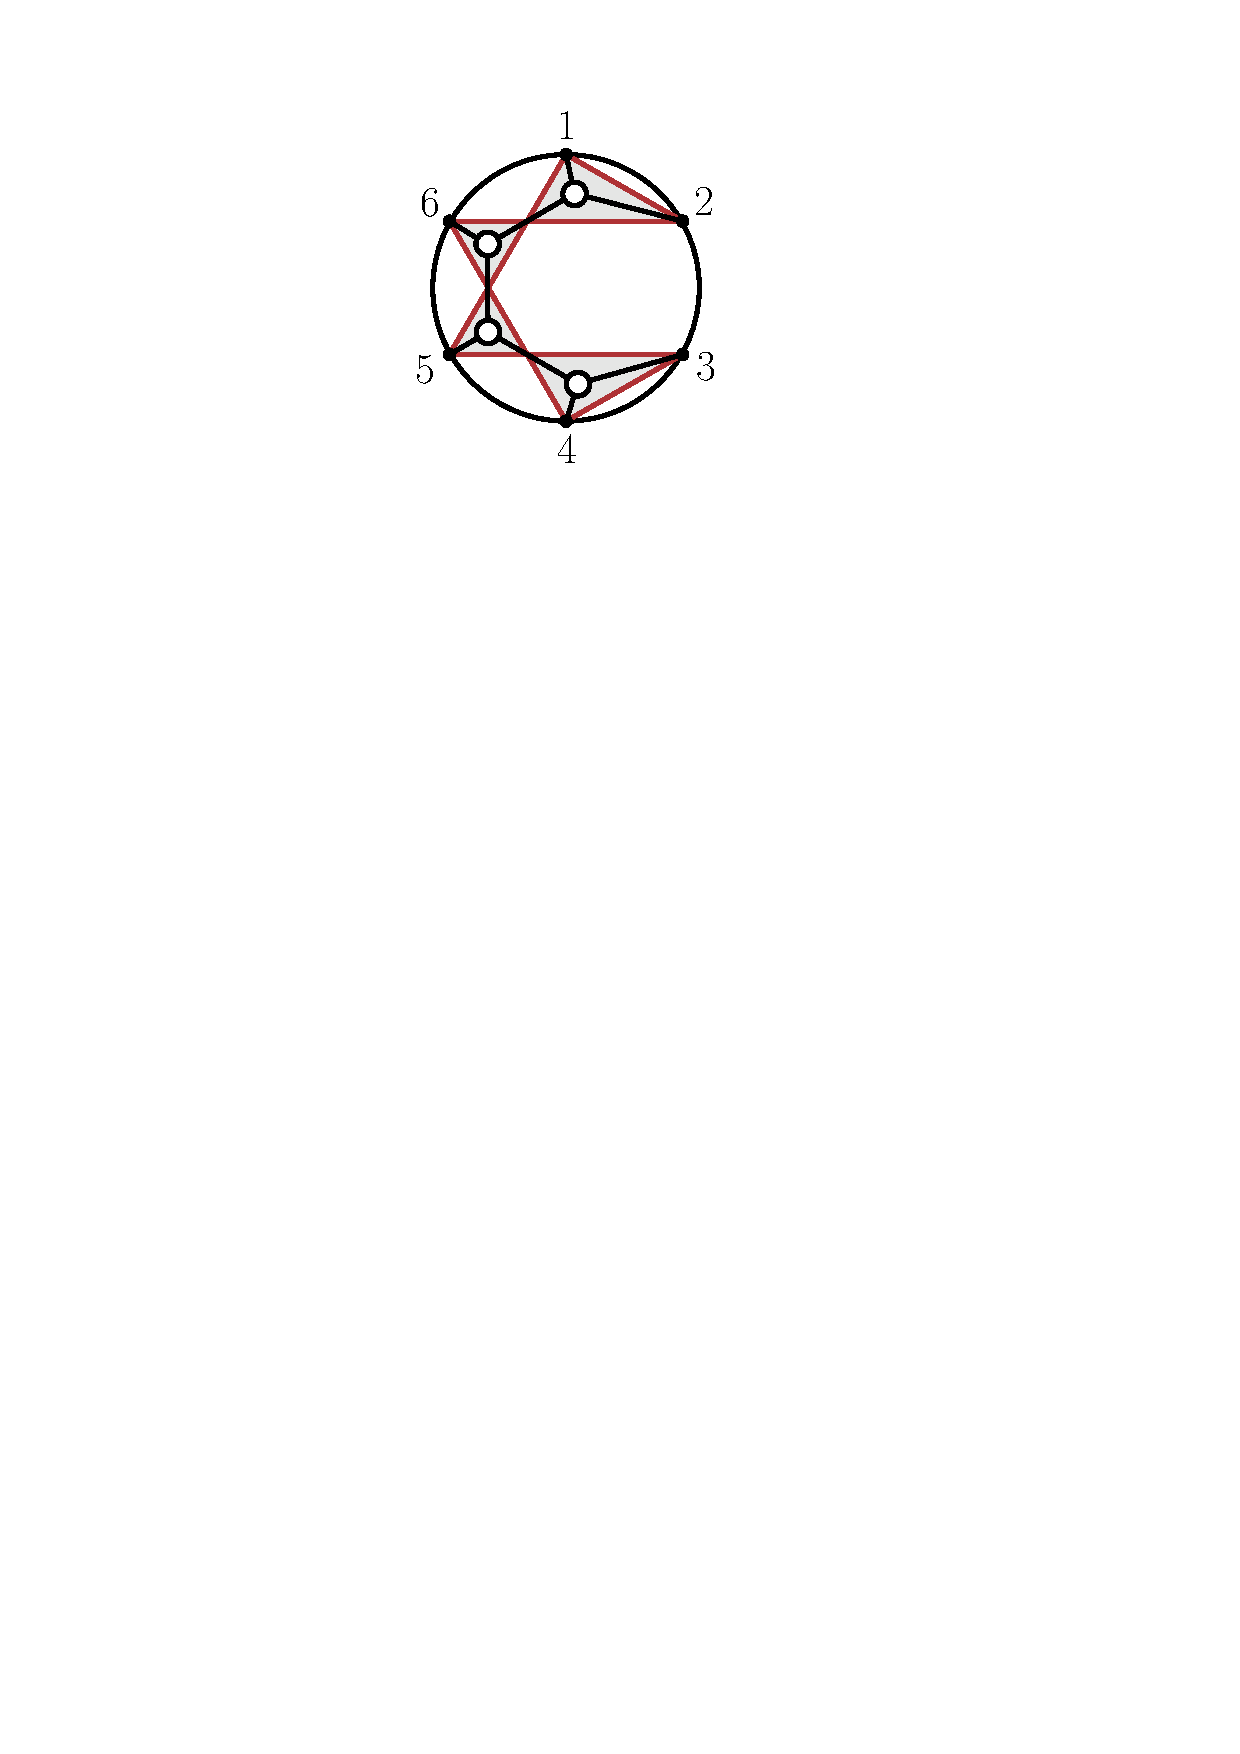
\includegraphics[scale=.5]{figs/eqfig1.pdf}} =\, \frac{1}{\sin s_{12} \,\sin s_{34} \,\sin s_{345}}
\end{equation}
\begin{equation}
\begin{aligned}
		m_{\alpha'}(\mathbb{I}_6|126345)\, &= \parbox[c]{6.5em}{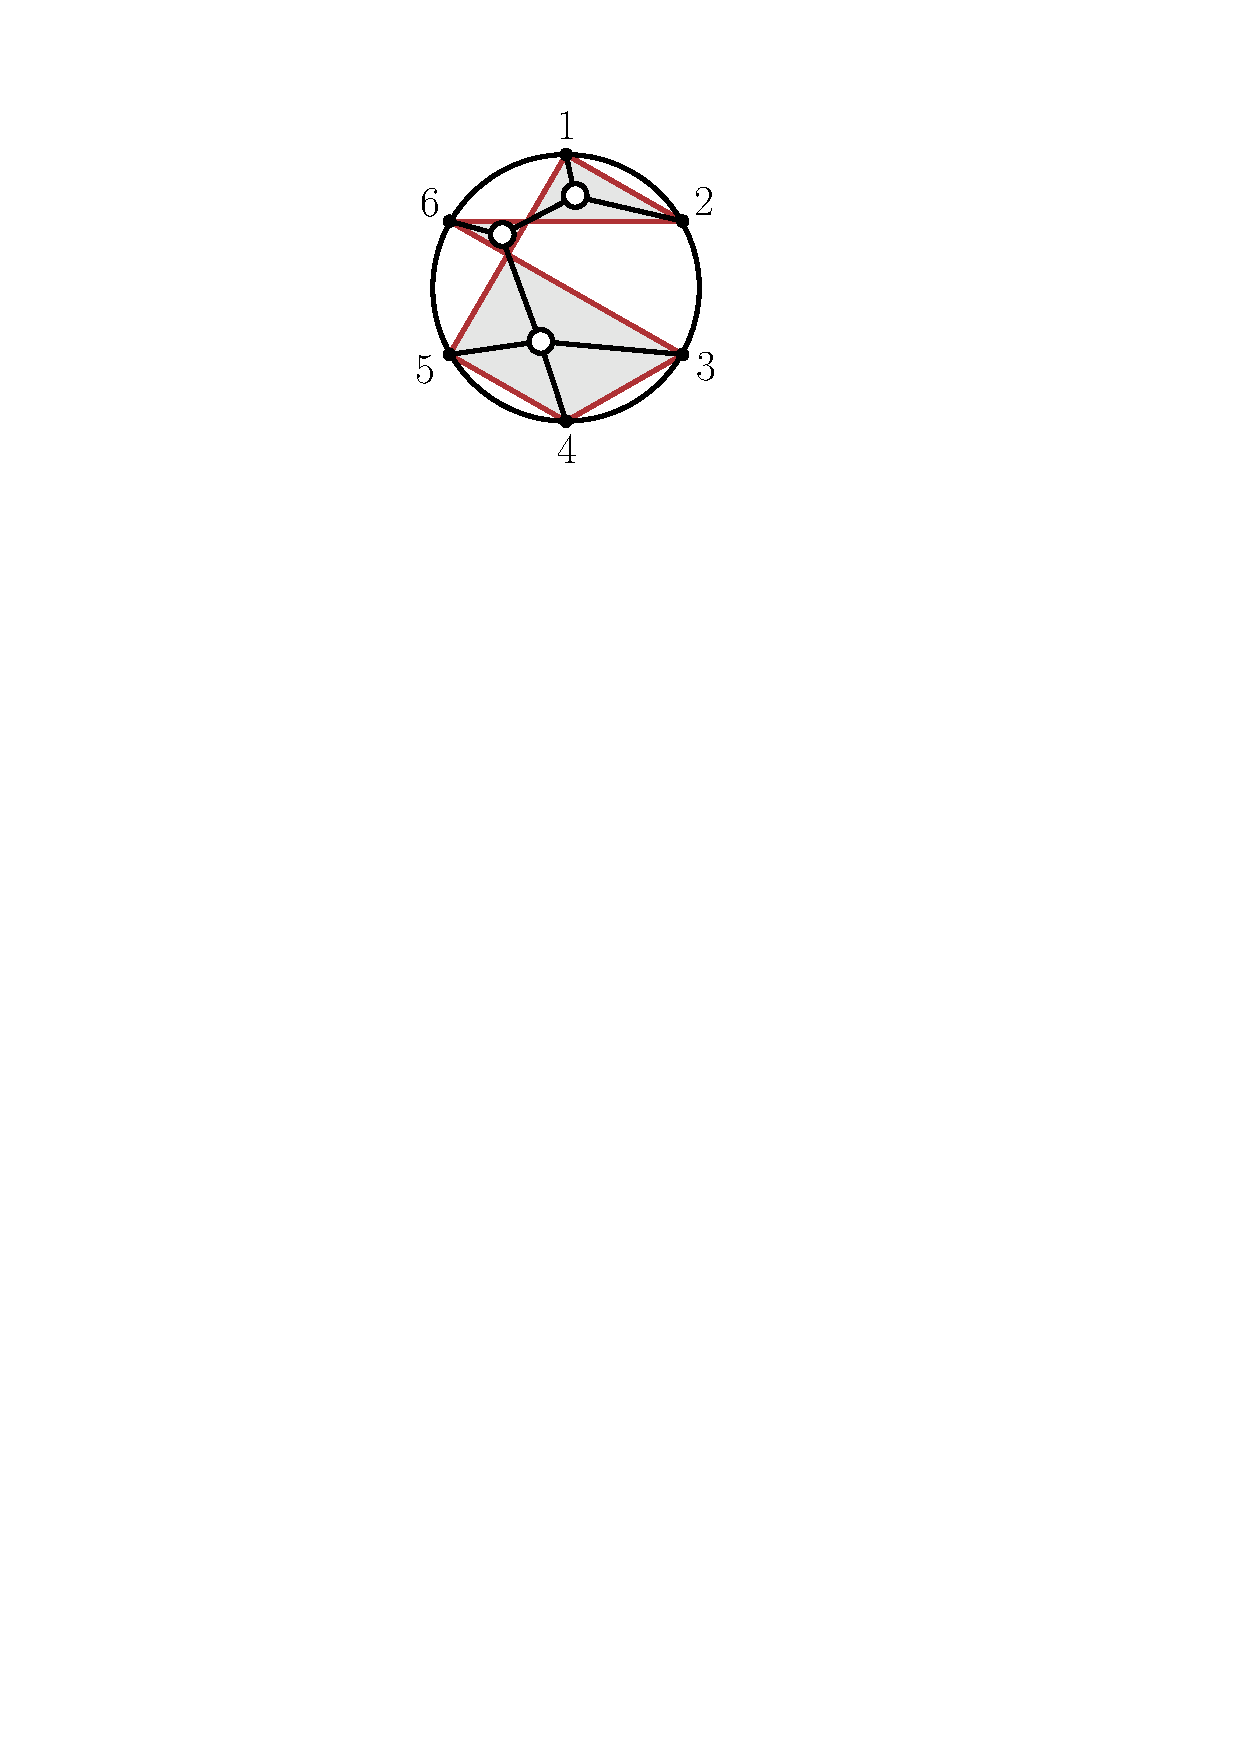
\includegraphics[scale=.5]{figs/m-123456-126345.pdf}} =\, -\frac{1}{\sin s_{12} \,\sin s_{612}} \times\!\!\! \parbox[c]{6.5em}{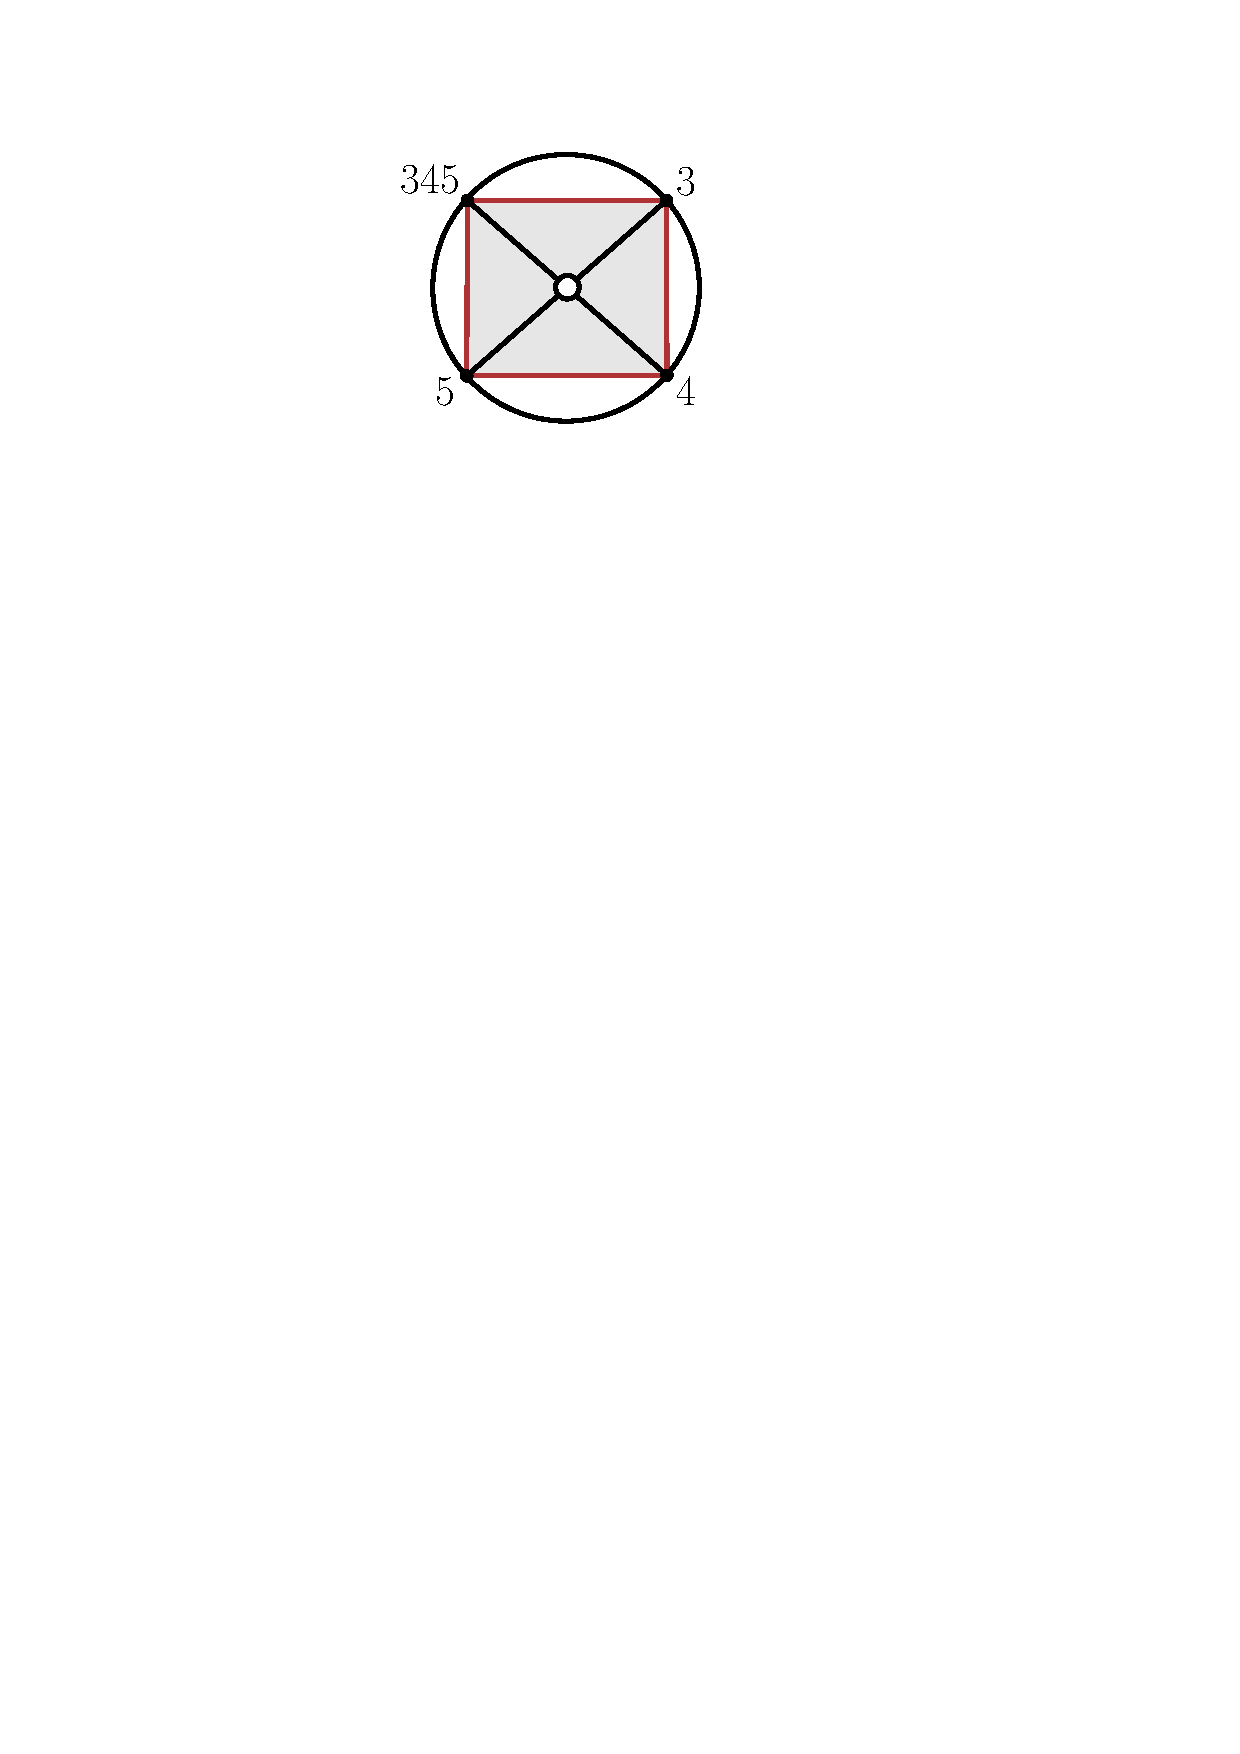
\includegraphics[scale=.5]{figs/m-123456-126345-small.pdf}}\\
	&=\, -\frac{1}{\sin s_{12} \,\sin s_{612}} \left(\frac{1}{\tan s_{34}} + \frac{1}{\tan s_{45}} \right)
\end{aligned}
\end{equation}

依赖上面两个式子我们来说明这一图形规则,首先计算$\alpha\neq\beta$,他们可以展开成$\alpha=\beta$的情况。展开方法就是先按照$\alpha$的顺序在盘面上把点标记出来,然后再按照$\beta$的顺序连接,也就是上图的红线,如果这一步给出的不是平面图,比如$m_{\alpha'}(12345|13524)$一样的五角星,那么就直接是$0$。这些红线会交出多边形,每个多边形内部画一个白点,白点之间连接,给出传播子$1/\sin(s_e)$,白点和多边形顶点相连,相当于动量外腿。每个多边形看作这种费曼规则的一个顶点,他们就贡献$m_{\alpha'}(\mathcal{E}|\mathcal{E})$,$\mathcal{E}$表示顶点边上动量外腿的集合。前面的正负号由缠绕数的计算给出$(-1)^{w(\alpha|\beta)+1}$:
\begin{equation}
	w(\mathbb{I}_6 | 126345)\, = \parbox[c]{6.5em}{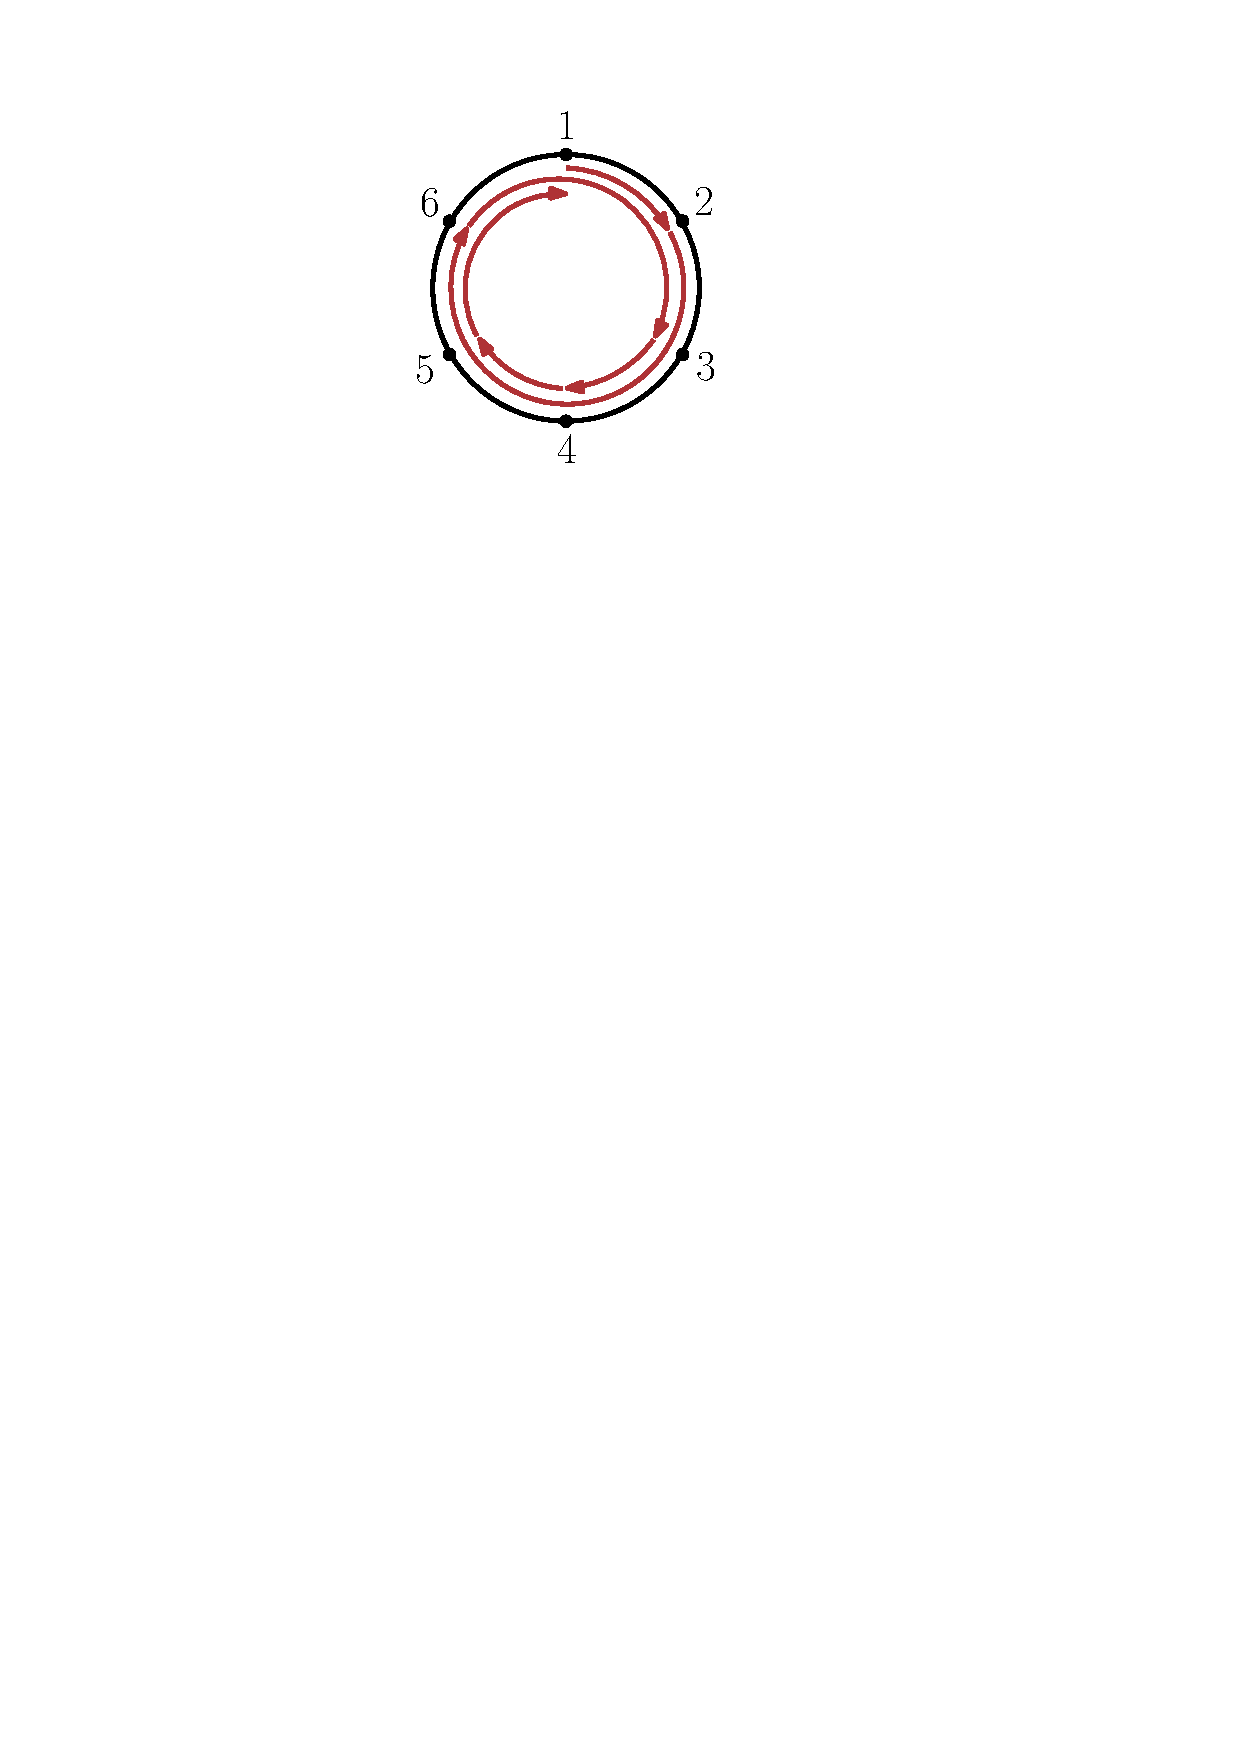
\includegraphics[scale=.5]{figs/wrapping.pdf}}\, =\, 2
\end{equation}
也就是说,缠绕数计算就是按照$\beta$的顺序缠绕$\alpha$得来。然后计算对角部分,也就是那些“顶点”项,以$\alpha=\beta=\mathbb{I}_n$为例,剩下的可以通过置换下标得到:
\begin{equation}
\begin{aligned}
		m_{\alpha'}(\mathbb{I}_5 | \mathbb{I}_5 )\, =\,& \parbox[c]{6.5em}{\vspace{-.5em}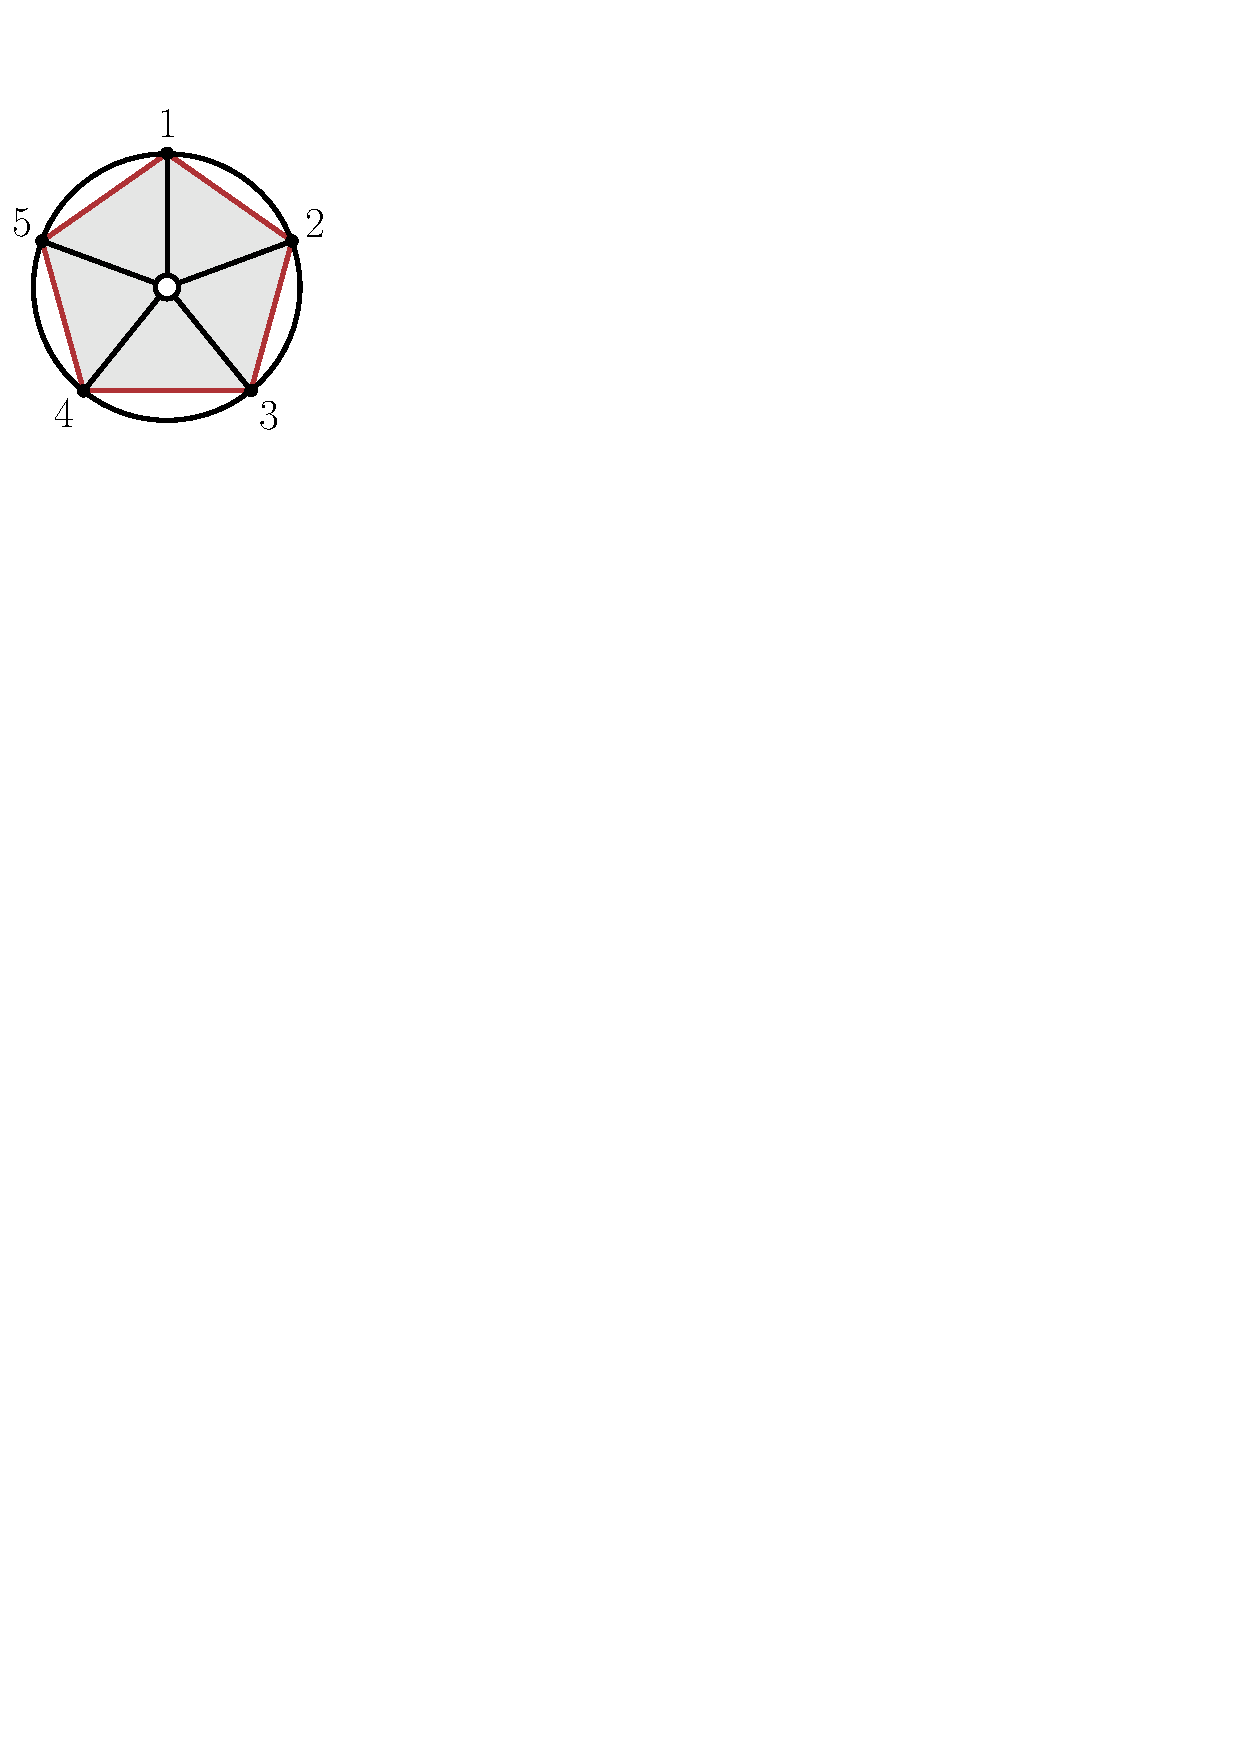
\includegraphics[scale=.5]{figs/m-12345-12345}}\, =\begin{aligned}
			\parbox[c]{6em}{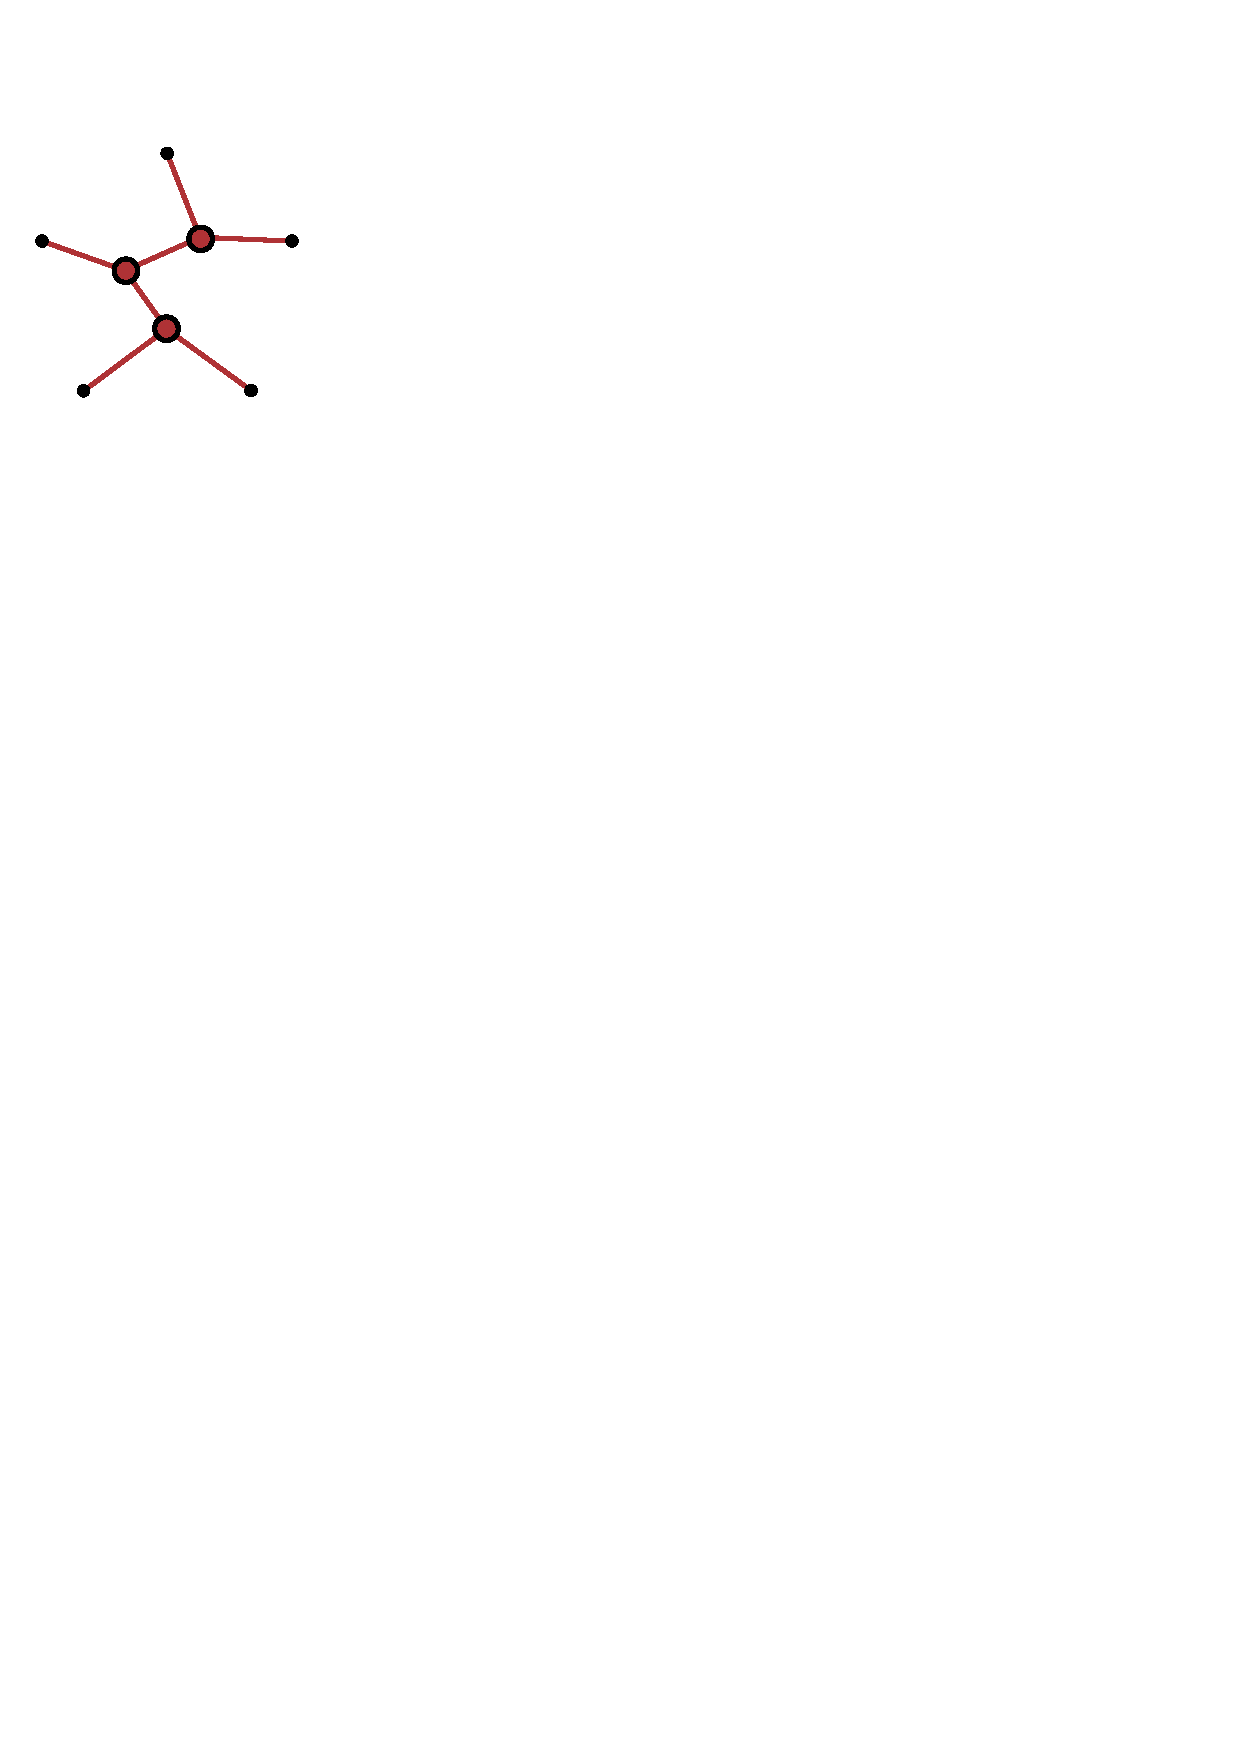
\includegraphics[scale=.5]{figs/m-12345-12345-a}}\, + \,\parbox[c]{6em}{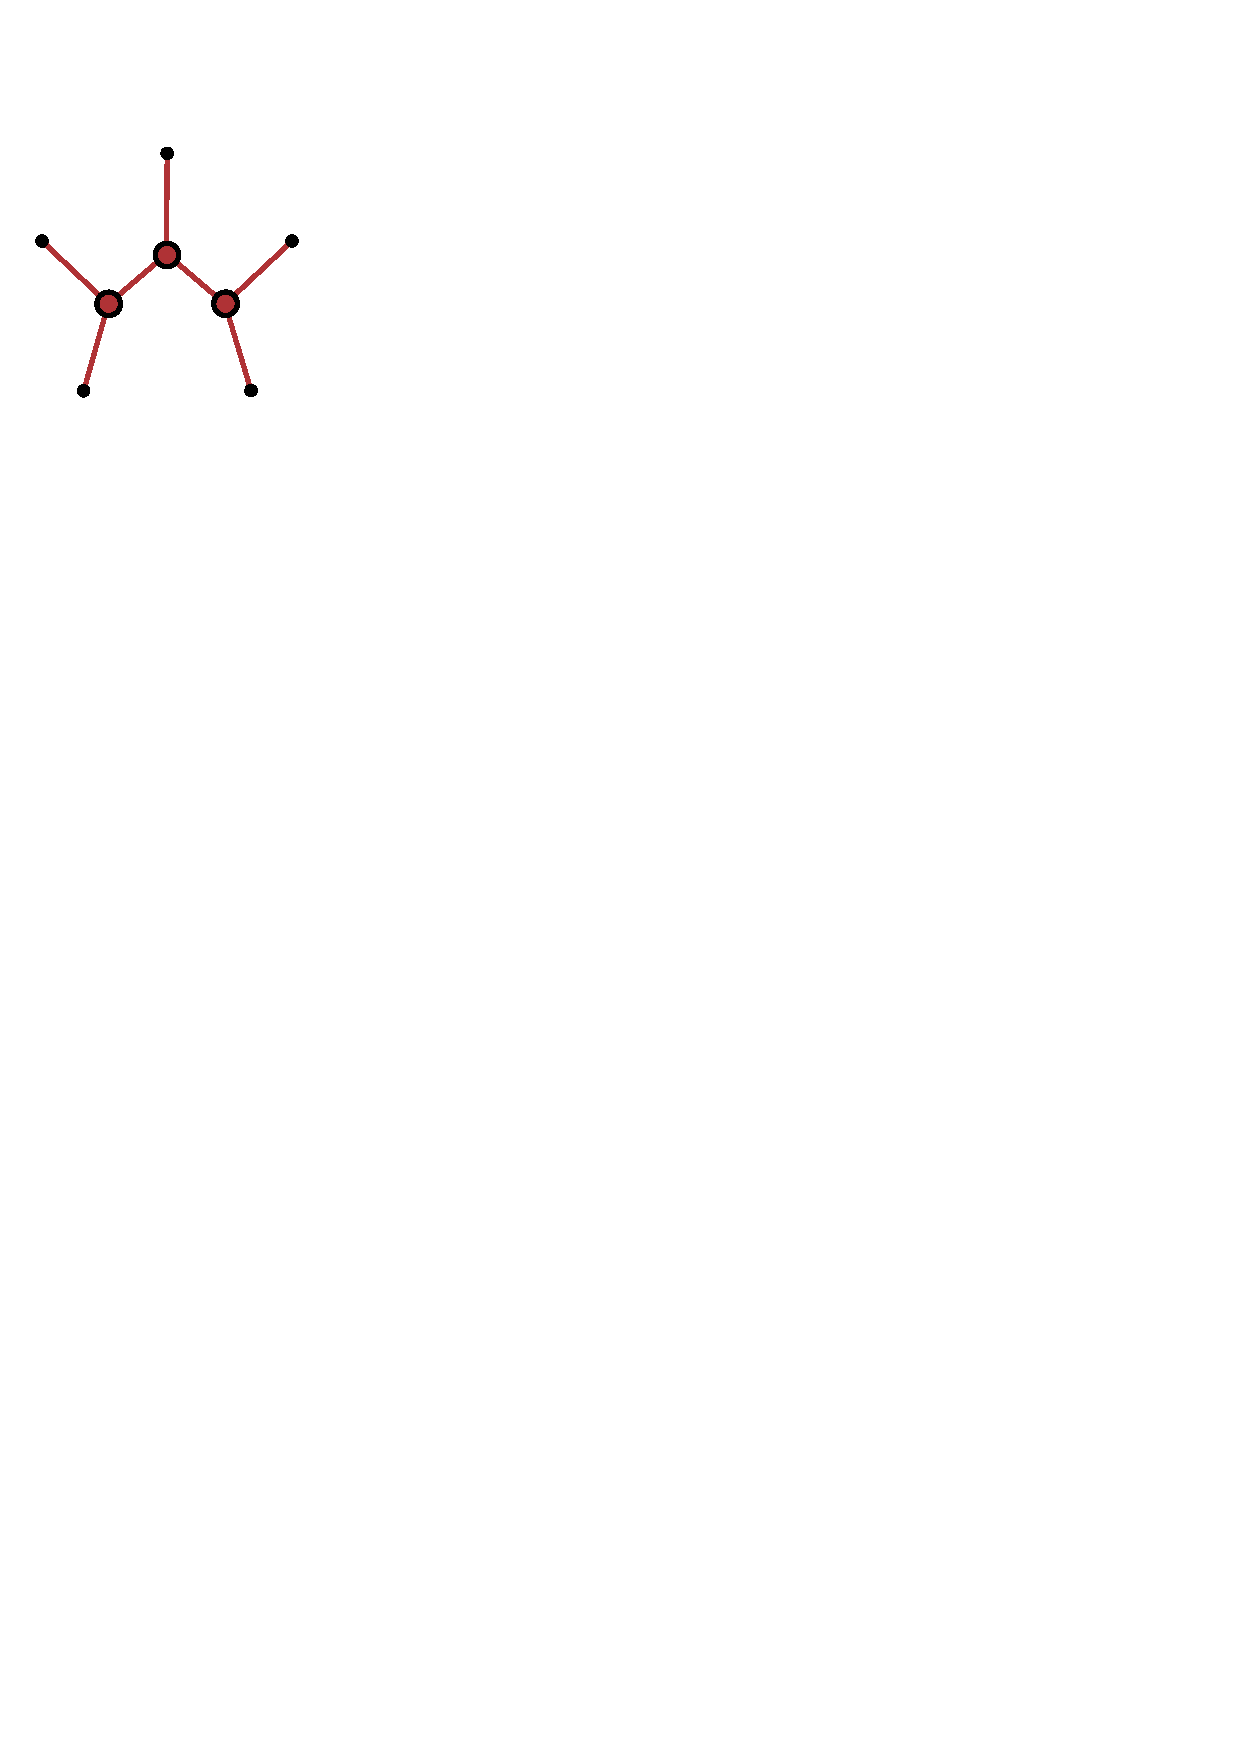
\includegraphics[scale=.5]{figs/m-12345-12345-b}}\, +\, \parbox[c]{6em}{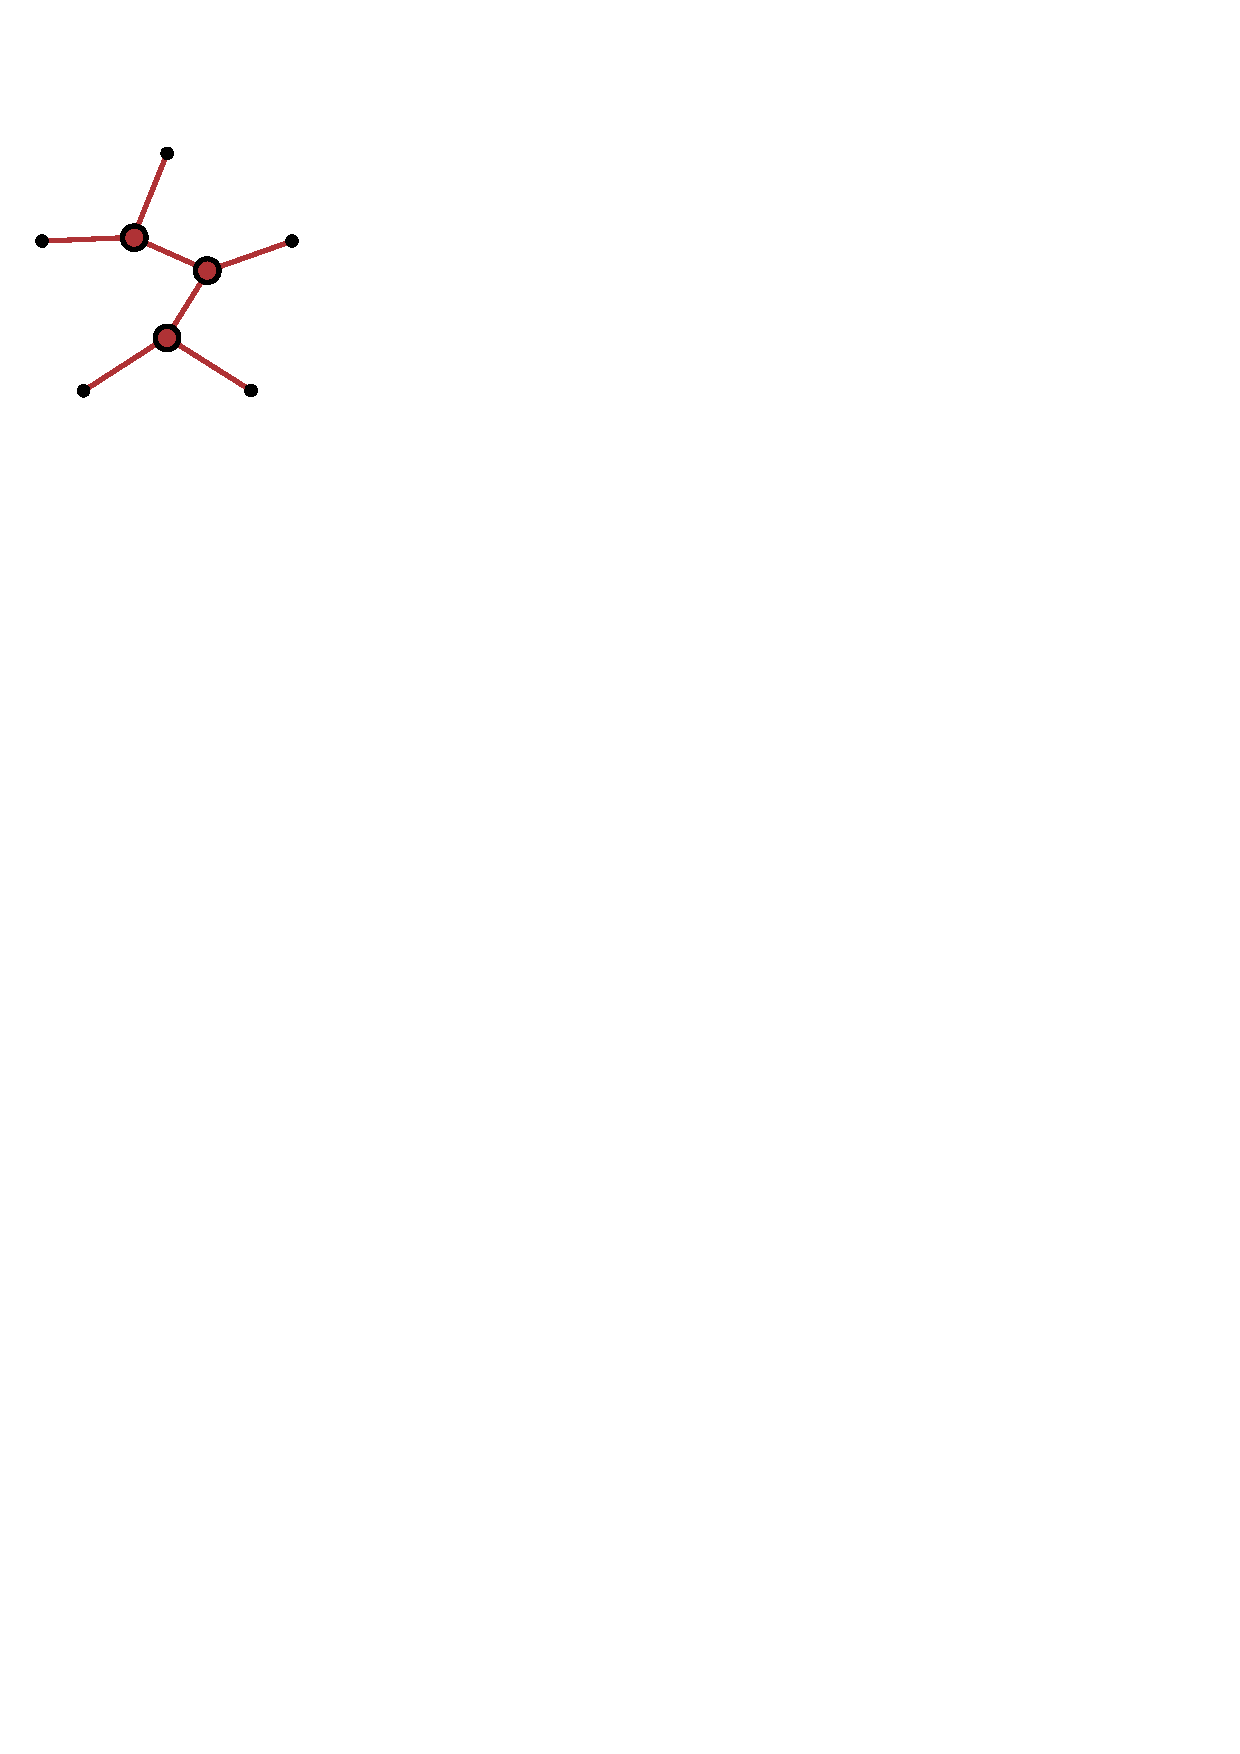
\includegraphics[scale=.5]{figs/m-12345-12345-c}} \\
			+\, \parbox[c]{6em}{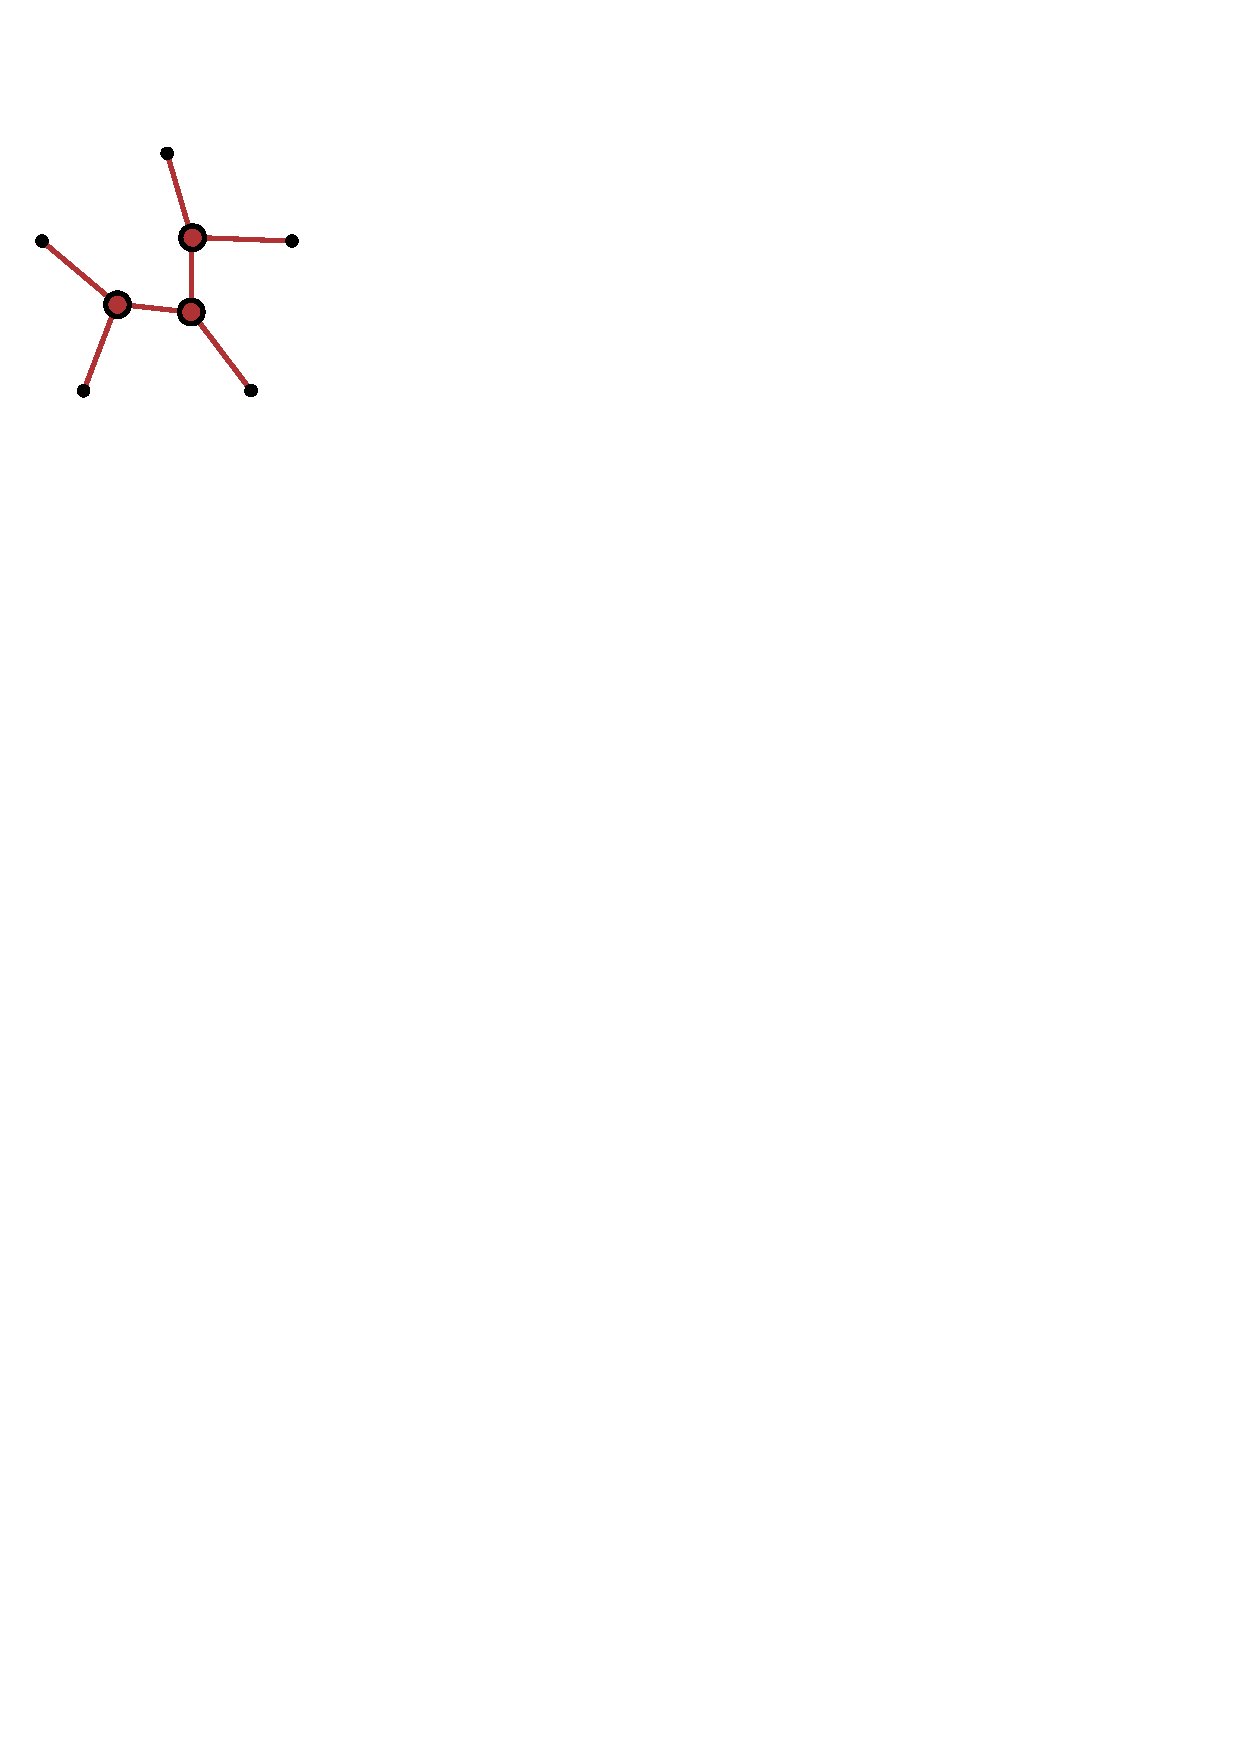
\includegraphics[scale=.5]{figs/m-12345-12345-d}}\, +\, \parbox[c]{6em}{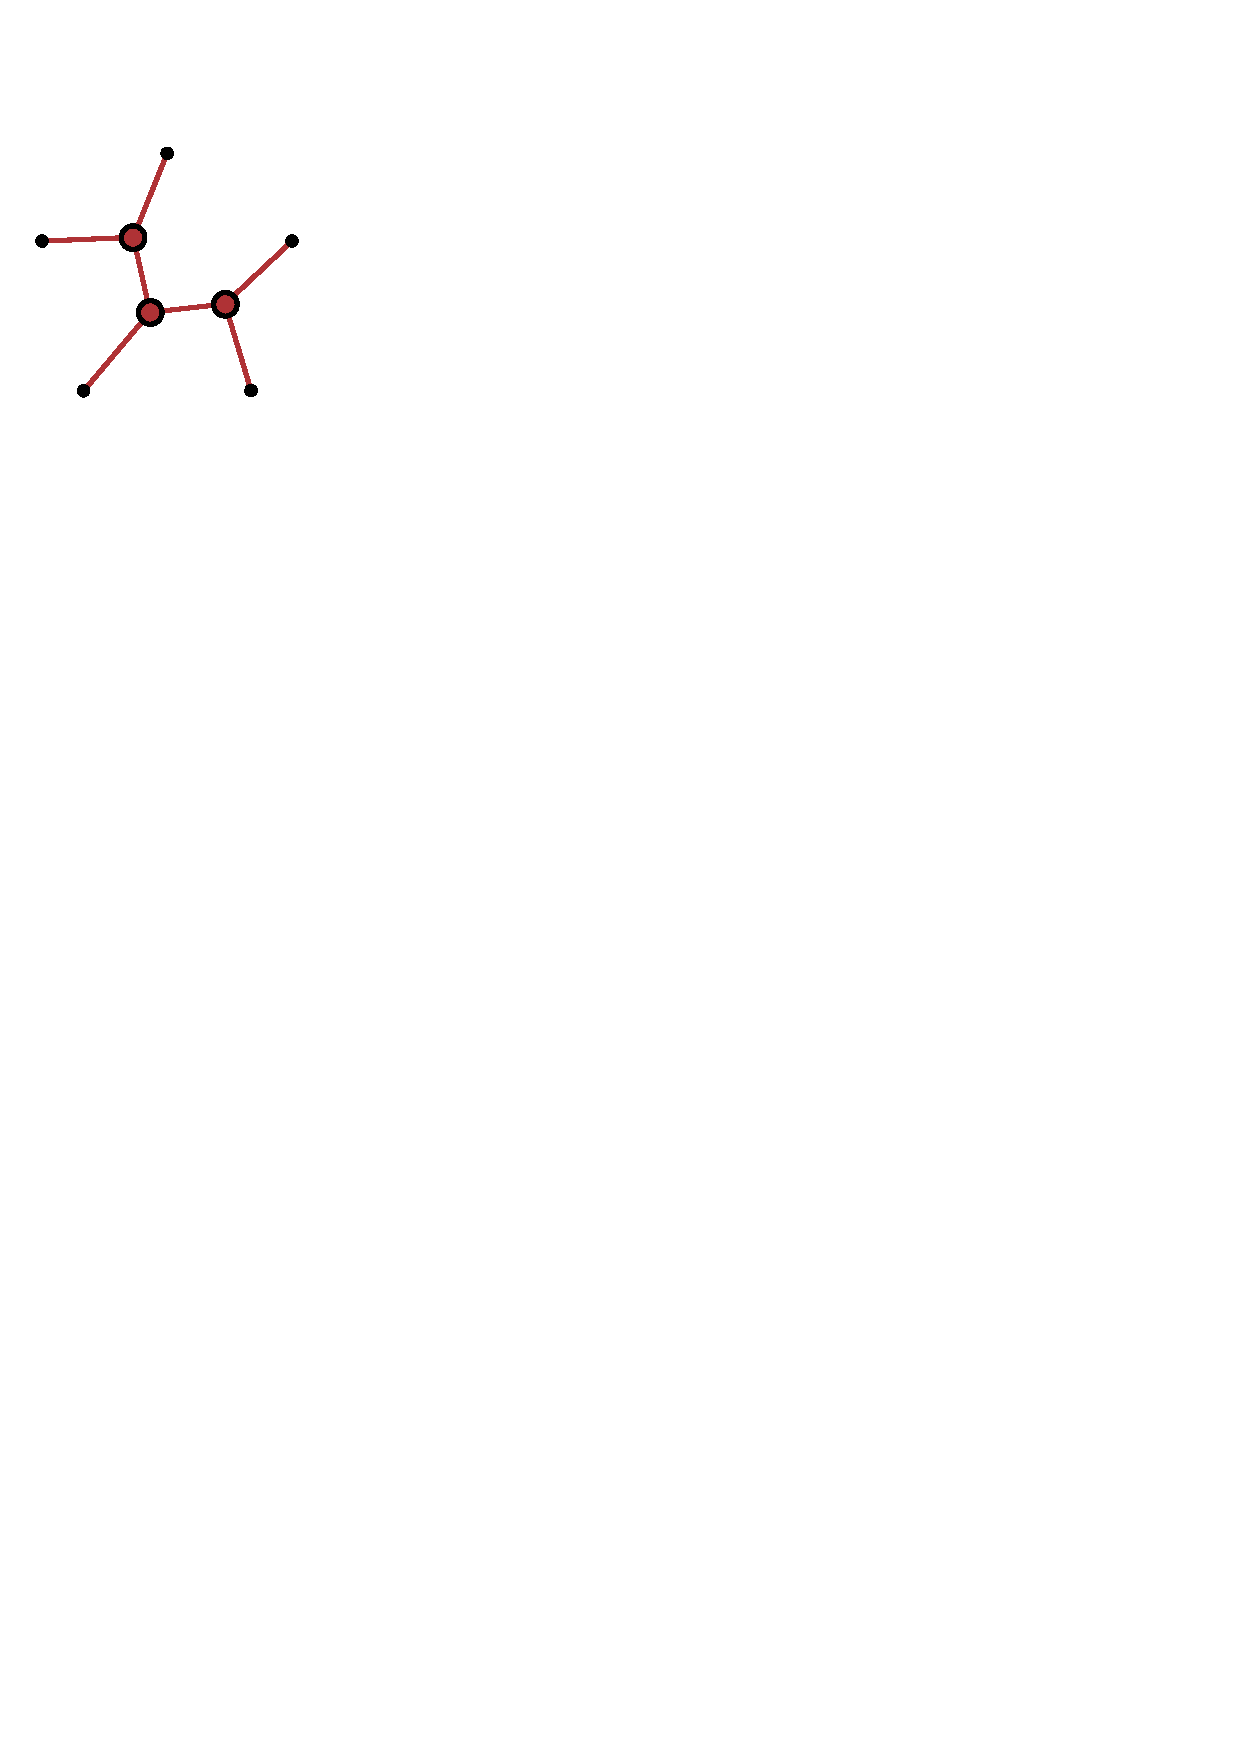
\includegraphics[scale=.5]{figs/m-12345-12345-e}} \,+\, \parbox[c]{6em}{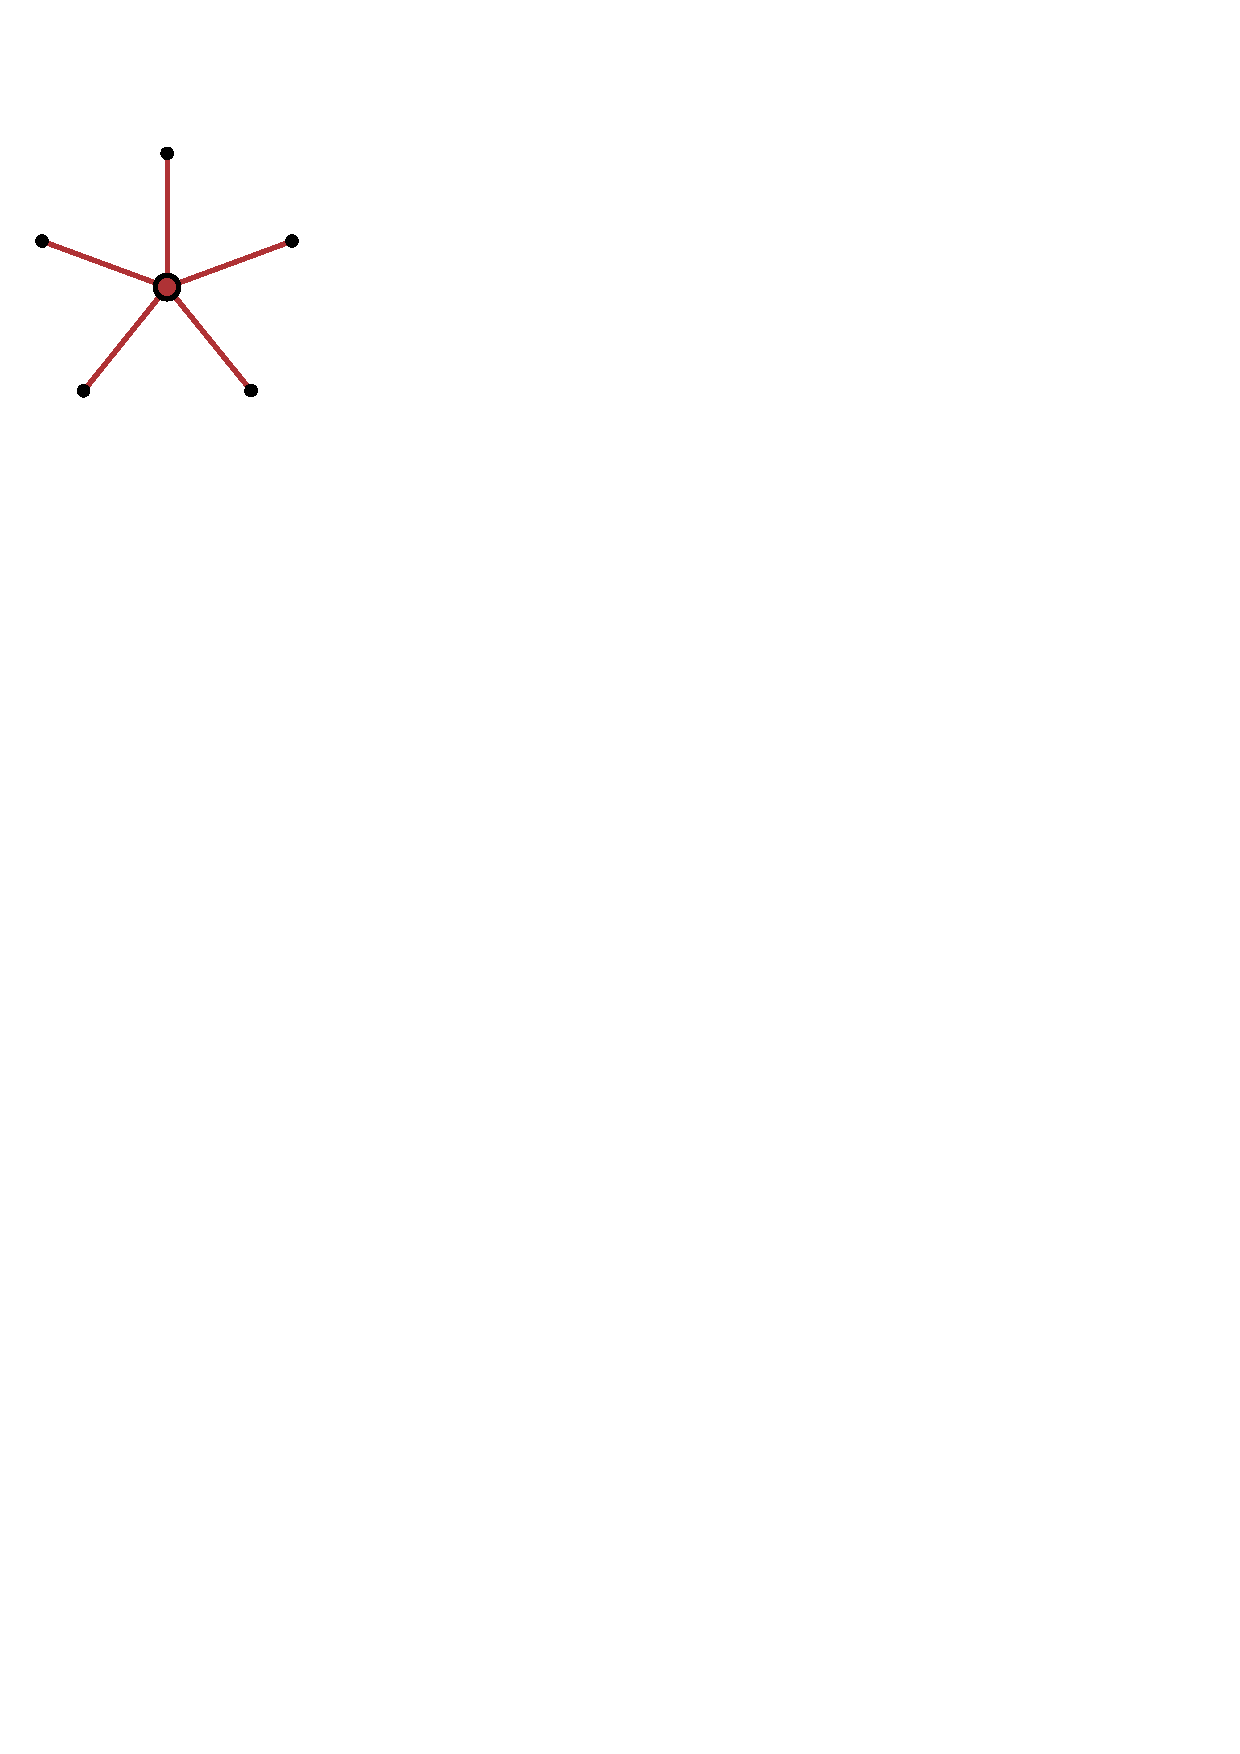
\includegraphics[scale=.5]{figs/m-12345-12345-f}} \\
		\end{aligned} \\
	=& \quad\frac{1}{\tan s_{12}\, \tan s_{34}} + \frac{1}{\tan s_{23}\, \tan s_{45}} + \frac{1}{\tan s_{34}\, \tan s_{51}} 
	 + \frac{1}{\tan s_{45}\, \tan s_{12}} \\
	 &+ \frac{1}{\tan s_{51}\, \tan s_{23}} + 1
\end{aligned}
\end{equation}
也就是说首先画出所有外腿顺序固定的所有用奇数外腿顶点构造的费曼图,每个顶点项贡献:
\begin{equation}
	\parbox[c]{8em}{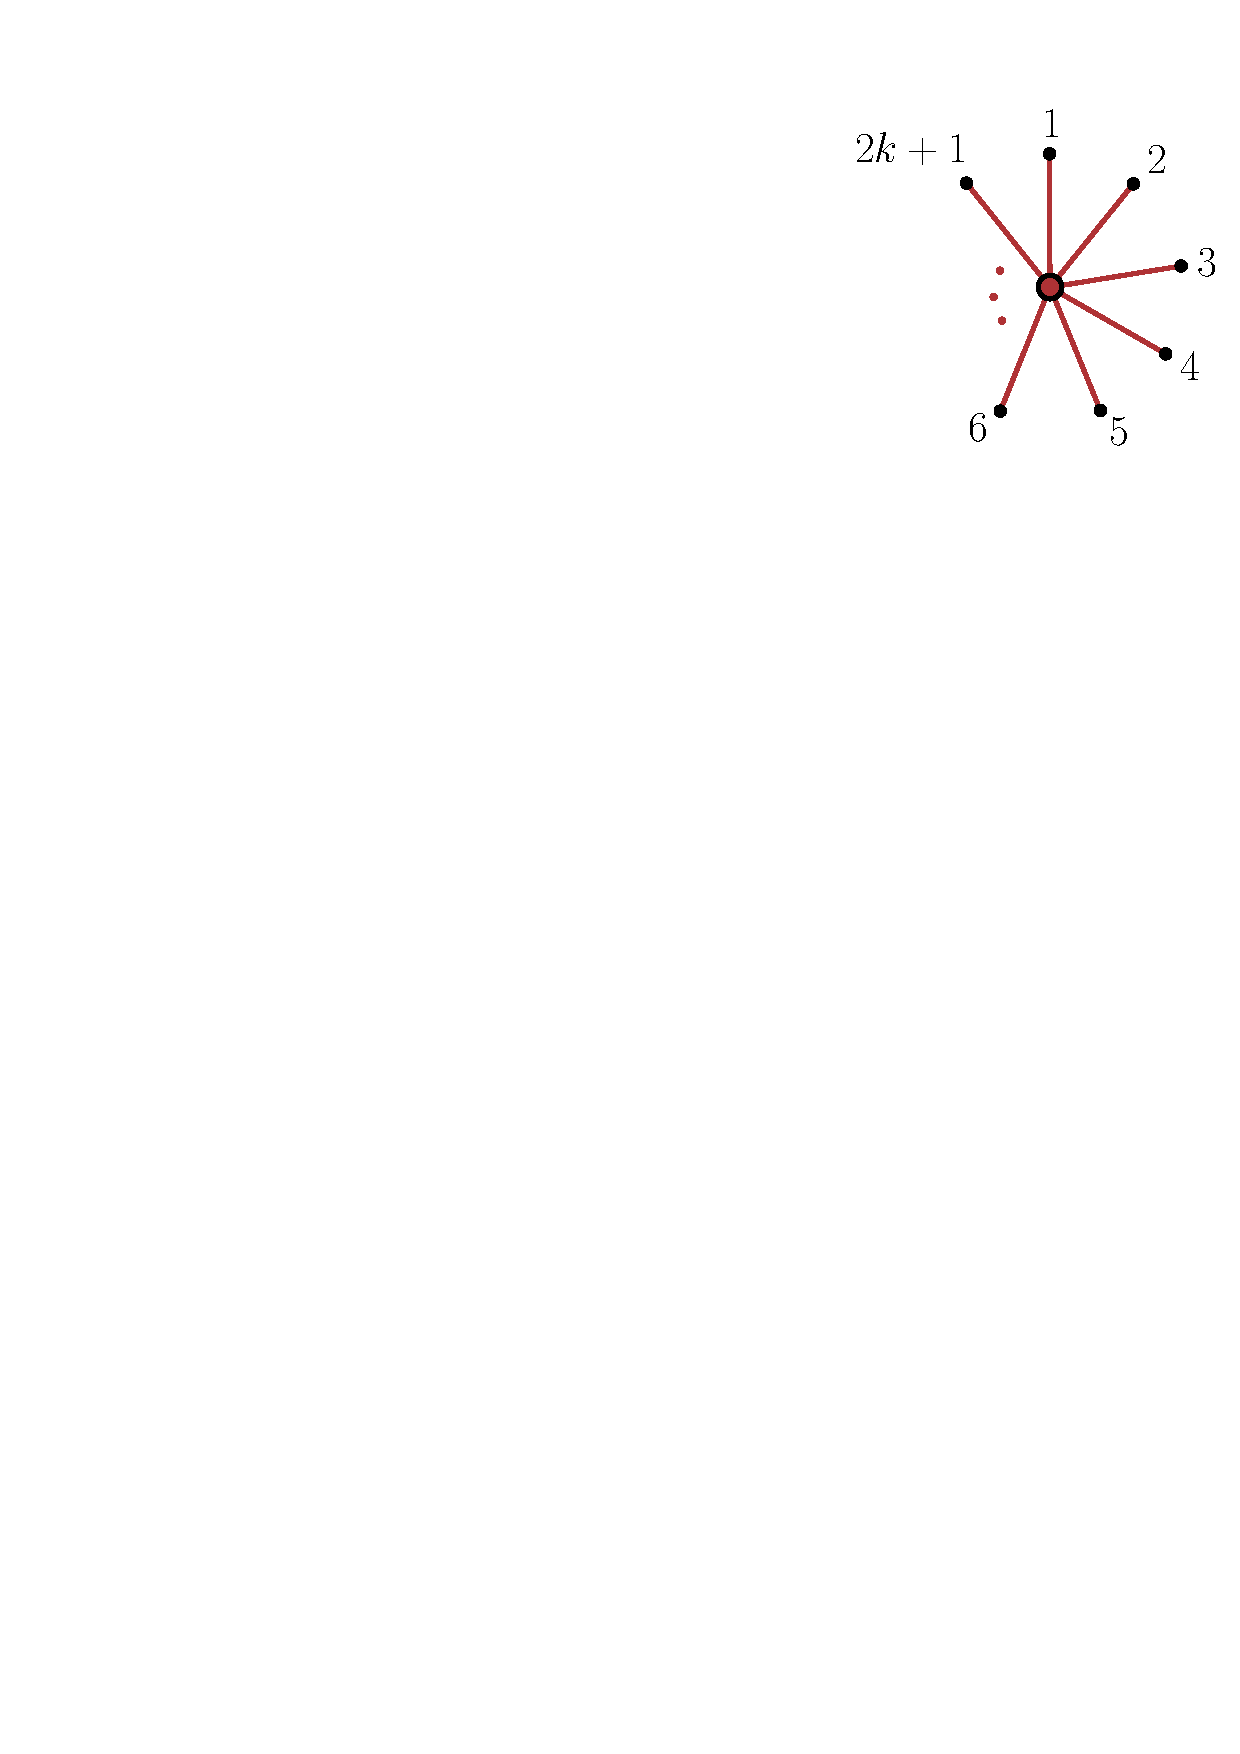
\includegraphics[scale=.5]{figs/m-vertex}}\; = \; C_{k-1}
\end{equation}
$C$是Catalan数。而每个传播子贡献$1/\tan(s_e)$。然后对$m_{\alpha'}$取逆矩阵就得到需要的KLT矩阵。上述色序振幅可以对应到一个场论,所以KLT关系实际上在说:
\begin{equation*}
	\text{Closed string}=\frac{\text{Open string}^2}{\alpha^{\prime}\text{-corrected bi-adjoint scalar}}
\end{equation*}

KLT关系实际上依赖于球面上左右模独立传播的特性,这一点在$\mathbb{RP}^2$上并不成立,所以无法分解为盘面振幅\cite{dyj}。文献\cite{Kawai:1985xq}中特别对四点情况KLT关系进行了详细论证。规范固定后四点KLT核只有一项,所以:
\begin{equation}
	\mathcal{M}_4 \sim-\frac{\sin(\pi s_{12})}{2\pi\alpha^{\prime}}A_4(1,2,3,4)\tilde A_4(1,2,4,3)
\end{equation}
不难发现这正是振幅\ref{Veneziano}和\ref{eq:4.45}之间的联系。\footnote{计算中需要用到$\sin(\pi x) = \frac{-\pi}{\Gamma(x+1)\Gamma(-x)}$。}
\section{RNS超弦振幅}
\subsection{自旋场关联函数}
在计算涉及R部分激发态时,会用到自旋场。回忆一下用OPE计算关联函数,首先用Wick定理计算多点OPE看出奇异性,而树图关联函数又只依赖于这种奇异性,所以可以直接用Wick收缩得到关联函数。但是,观察自旋场OPE,我们发现R部分并不是一个自由CFT,也就是说OPE得到的结果仍然包含场算符。对于非自由CFT,原先使用的Wick定理这些都失效了,本身关联函数相较于OPE也多了不少信息,但是,至少对于两个自旋场插入情况,我们可以利用OPE得知的关联函数奇异性信息完全从两点三点关联函数自举$n$点振幅。根据$\psi$和$S_A$都是共形主场,再根据他们的指标($SO(D-1,1)$表示)类型可以完全确定两点三点关联函数:
\begin{equation}
	\label{eq:4.61}
	\langle\psi^\mu(z_1)S_A(z_2)S_B(z_3)\rangle=\frac{(\Gamma^\mu\mathcal{C})_{AB}}{\sqrt{2}z_{12}^{1/2}z_{13}^{1/2}z_{23}^{D/8-1/2}},\quad \left\langle{S_{A}(z_1)S_{B}(z_2)}\right\rangle=\frac{\mathcal{C}_{AB}}{(z_1-z_2)^{D/8}}
\end{equation}
这是共形场论中熟知的结论,GSO投影将R部分真空投影到Weyl旋量,所以有如下的分解:\footnote{$\mathcal{C}_{AB}$的分解与时空维数有关,这里是$2\mod 4$的情况,而对$2\mod 4$,分解为$\mathcal{C}_{AB}=\begin{pmatrix}C_{\alpha\beta}&0\\0&C^{\dot{\alpha}\dot{\beta}}\end{pmatrix}$。}
\begin{equation}
	\label{eq:4.65}
	S_A=\begin{pmatrix}S_\alpha\\S^{\dot{\alpha}}\end{pmatrix},\quad(\Gamma^\mu)_A{}^B=\begin{pmatrix}0&\gamma_{\alpha\dot{\beta}}^\mu\\\bar{\gamma}^{\mu\dot{\alpha}\beta}&0\end{pmatrix},\quad \mathcal{C}_{AB}=\begin{pmatrix}0&{C_{\alpha}}^{\dot{\beta}}\\{C^{\dot{\alpha}}}_{\beta}&0\end{pmatrix}
\end{equation}
后面开弦计算只会用到其中一个手性,比如$S_\alpha$,$\gamma^\mu_{\alpha\dot\beta}$和${C_{\alpha}}^{\dot\beta}$。我们以四点为例说明如何计算球面上的关联函数。首先根据其指标结构可以写下一般的拟设:
\begin{equation}
	\langle\psi^\mu(z_1)\psi^n(z_2)S_A(z_3)S_B(z_4)\rangle=\eta^{\mu\nu}\mathcal{C}_{AB}f(\mathbf{z})+\frac{1}{2}(\Gamma^\mu\Gamma^\nu\mathcal{C})_{AB}g(\mathbf{z})
\end{equation}
然后根据OPE领头阶得到如下奇异行为:
\begin{equation}
	\langle\psi^\mu(z_1)\psi^\nu(z_2)S_A(z_3)S_B(z_4)\rangle\to
	\begin{cases}\frac{\eta^{\mu\nu}}{z_m}\langle S_A(z_3)S_B(z_4)\rangle&, z_1\to z_2\\\frac{{{\Gamma^{\mu}}_A}^C}{\sqrt{2}z_{13}^{1/2}}\langle\psi^n(z_2)S_C(z_3)S_B(z_4)\rangle&, z_1\to z_3\\\frac{{{\Gamma^{\mu}}_B}^C}{\sqrt{2}z_{14}^{1/2}}\langle\psi^n(z_2)S_A(z_3)S_C(z_4)\rangle&, z_1\to z_4
	\end{cases}
\end{equation}
再利用关联函数\ref{eq:4.61}得到:
\begin{equation}
	\begin{aligned}
		&f(\mathbf{z})\to\begin{cases}z_{12}^{-1}z_{34}^{-D/8}&,z_1\to z_2\\\mathrm{regular}&,z_1\to z_3\\(z_{14}z_{23}z_{24})^{-1/2}z_{34}^{1/2-D/8}&,z_1\to z_4\end{cases}\\
		&g(\mathbf{z})\to\begin{cases}\mathrm{regular}&,z_1\to z_2\\(z_{13}z_{23}z_{24})^{-1/2}z_{34}^{1/2-D/8}&,z_1\to z_3\\(z_{14}z_{23}z_{24})^{-1/2}z_{34}^{1/2-D/8}&,z_1\to z_4\end{cases}
	\end{aligned}
\end{equation}
根据黎曼面上半纯函数都是有理形式,由上面奇异性直接得到:
\begin{equation}
	f(\mathbf{z})=\frac{z_{13}z_{24}}{z_{12}(z_{13}z_{14}z_{23}z_{24})^{1/2}z_{34}^{D/8}},\quad g(\mathbf{z})=\frac{1}{(z_{13}z_{14}z_{23}z_{24})^{1/2}z_{34}^{D/8-1}}
\end{equation}
从而有四点关联函数:
\begin{equation}
	\langle\psi^\mu(z_1)\psi^\nu(z_2)S_A(z_3)S_B(z_4)\rangle=\frac{z_{34}^{1-D/8}}{(z_{13}z_{14}z_{23}z_{24})^{1/2}}\left(\frac{z_{13}z_{24}}{z_{12}z_{34}}\eta^{\mu\nu}\mathcal{C}_{AB}+\frac{1}{2}(\Gamma^\mu\Gamma^\nu\mathcal{C})_{AB}\right)
\end{equation}
更高点的完全类似,只是拟设更为复杂,但是思想就是利用OPE读出奇异性,然后发现奇异性本身就足以和拟设一起完全确定关联函数。更多自旋场的插入需要更多纯自旋场关联函数,但是其计算非常复杂,结果需要用$\Theta$函数相关的复杂表达式,圈图推广以及更一般性的讨论详见文献\cite{Schlotterer:2012zz,Hartl:2011tza,Haertl:2011yvw}及其所引文献。
\subsection{振幅的计算}
由于球面超弦振幅同样可以根据KLT关系用盘面超弦振幅表达,所以这里只计算一些简单的盘面超弦振幅。首先是三胶子振幅:
\begin{equation}
	\label{eq:4.71}
	\begin{aligned}
		A_3(\epsilon_1,\epsilon_2,\epsilon_3)=&|z_{12}z_{13}z_{23}|\langle U^{(0)}(z_1)U^{(-1)}(z_2)U^{(-1)}(z_3)\rangle\\
		\sim&|z_{12}z_{13}z_{23}|\langle:e^{-\phi(z_2)}::e^{-\phi(z_3)}:\rangle\epsilon_{1\mu}\epsilon_{2\nu}\epsilon_{3\lambda}\\
		&\times\left\{\left\langle :i\partial_{z_1}X^\mu(z_1)e^{ip_1\cdot X(z_1)}:\prod_{j=2}^3:e^{ip_j\cdot X(z_j)}: \right\rangle\left\langle\psi^\nu(z_2)\psi^\lambda(z_3)\right\rangle\right.\\
		&+2\alpha'\left\langle\prod_{j=1}^3:e^{ip_j\cdot X(z_j)}:\right\rangle p_{1\rho}\left\langle:\psi^\rho\psi^\mu(z_1):\psi^\nu(z_2)\psi^\lambda(z_3)\right\rangle\bigg\}\\
		\sim&\cancelto{-1}{\frac{|z_{12}z_{13}z_{23}|}{z_{12}z_{13}z_{23}}}\left[(p_2\cdot\epsilon_1)(\epsilon_2\cdot\epsilon_3)+(\epsilon_1\cdot\epsilon_2)(p_1\cdot\epsilon_3)-(\epsilon_1\cdot\epsilon_3)(p_1\cdot\epsilon_2)\right]\\
		=&A_{\mathrm{SYM}}(\epsilon_1,\epsilon_2,\epsilon_3)
	\end{aligned}
\end{equation}
注意这里$|z_{1,2,3}|/z_{1,2,3}$的项取$\pm1$和色序有关,另外一个$(132)$的色序给出$+1$\footnote{所以如果没有色序,其实三胶子振幅直接就是$0$,这对应QED中没有三光子顶点。}。其中玻色场关联函数已在\ref{eq:4.37}中给出,剩下的自由费米子关联函数直接用OPE计算全部外腿Wick缩并即可,比如:
\begin{equation}
\begin{aligned}
		\left\langle:\psi^\rho\psi^\mu(z_1):\psi^\nu(z_2)\psi^\lambda(z_3)\right\rangle 
	&=\wick{\left\langle:\c1\psi^\rho\c2\psi^\mu:\c1\psi^\nu\c2\psi^\lambda\right\rangle} +\wick{\left\langle:\c1\psi^\rho\c2\psi^\mu:\c2\psi^\nu\c1\psi^\lambda\right\rangle} \\
	&=\frac{\eta^{\mu\nu}\eta^{\rho\lambda}-\eta^{\mu\lambda}\eta^{\rho\nu}}{z_{12}z_{13}}
\end{aligned}
\end{equation}
这里$A_{\text{SYM}}$表示十维超对称Yang-Mills理论的色序振幅,由下面拉格朗日量计算,$C$是荷共轭矩阵,$[D_\mu,\chi]:=\partial_\mu\chi-[A_\mu,\chi]$:
\begin{equation}
	S_{\mathrm{SYM}}[A,\chi]\sim\int d^{10}X\operatorname{Tr}\left\{\frac{1}{4}F_{\mu\nu}F^{\mu\nu}+\chi^\alpha(\gamma^\mu C)_{\alpha\beta}[D_\mu,\chi^\beta]\right\}
\end{equation}
再比如一个胶子两个胶微子(gluino)的振幅:
\begin{equation}
	\label{eq:4.74}
	\begin{aligned}
		A_3(\epsilon_{1},u_{2},u_{3})\sim&|z_{12}z_{13}z_{23}|\langle U^{(-1)}(z_{1})U^{(-1/2)}(z_{2})U^{(-1/2)}(z_{3})\rangle\\
		=&|z_{12}z_{13}z_{23}|\langle:e^{-\phi(z_1)}::e^{-\phi(z_2)/2}::e^{-\phi(z_3)/2}:\rangle\langle\prod_{j=1}^3:e^{ip_j\cdot X(z_j)}:\rangle\\
		&\times\epsilon_1^\mu u_2^\alpha u_3^\beta\langle\psi_\mu(z_1)S_\alpha(z_2)S_\beta(z_3)\rangle\\
		\sim&\cancelto{-1}{\frac{|z_{12}z_{13}z_{23}|}{z_{12}z_{13}z_{23}}}\frac{1}{\sqrt{2}}\epsilon_1^\mu(u_2\gamma_\mu C u_3)\\
		=&A_{\text{SYM}}(\epsilon_1,u_2,u_3)
	\end{aligned}
\end{equation}

原则上来说,超对称理论的振幅应当是用格拉斯曼变量编码得到的超振幅,比如四维$\mathcal{N}=4$ SYM理论,超多重态自由度可以用格拉斯曼变量$\eta$编码到同一个波函数中表示,而分量振幅就根据超振幅的格拉斯曼变量次数来确定,比如:
\begin{equation}
	\label{eq:4.75}
\begin{gathered}
		A_n\left[S^{12}S^{34}3^-4^+\ldots n^+\right]=\left(\frac{\partial}{\partial\eta_{11}}\frac{\partial}{\partial\eta_{12}}\right)\left(\frac{\partial}{\partial\eta_{23}}\frac{\partial}{\partial\eta_{24}}\right)\left.\left(\prod_{A=1}^4\frac{\partial}{\partial\eta_{3A}}\right)\mathcal{A}_n[\Omega_1,\ldots,\Omega_n]\right|_{\eta_{kC}=0}\\
	\Omega=g^++\eta_A\lambda^A-\frac{1}{2!}\eta_A\eta_BS^{AB}-\frac{1}{3!}\eta_A\eta_B\eta_C\lambda^{ABC}+\eta_1\eta_2\eta_3\eta_4g^-
\end{gathered}
\end{equation}

因为胶子与胶微子共同构成一个超多重态,而前面计算那些振幅都应当是整个超振幅的某个分量振幅。但是由于RNS形式没有靶空间超对称,所以没办法直接计算超振幅。而且从前面三点振幅计算也能看出,超弦振幅和SYM振幅之间无论取外腿为超多重态中的哪一个态(胶子/胶微子),振幅之间的关系是不变的。而纯旋量超旋顶角算符直接对超多重态定义,所以可以直接计算得到超振幅,后面我们会用纯旋量超弦形式将任意多点盘面超弦超振幅表达为SYM超振幅。

另外对比玻色弦胶子振幅\ref{eq:4.47}和超弦胶子振幅\ref{eq:4.71},发现超弦振幅竟然更加简单,少了$\propto\alpha'$的项。缺少某一项从低能场论上看相当于低能场论缺少某个相互作用顶点。在场论中,超对称的引入一般能较好地改善理论的紫外行为,体现在超对称会直接否定某些抵消项的存在,比如在七圈以下修正,$\mathcal{N}=8$超引力只允许存在抵消项$R^4$,$D^4R^4$,$D^6R^4$\cite{Elvang:2015rqa}。这也是超弦振幅更加简单一些的一种解释。
